%--------------------------------------------------------------------
% Vorlage für eine Abschlussarbeit
% Darf ohne Einschränkungen weiterverwendet und abgeändert werden.
% mehr zur Verwedung in der README.md
% ⓒ (CC0) 2016, 2018 Henning Iseke <h_i_@online.de>
%--------------------------------------------------------------------

% Haupdatei

% Befehle für Metadaten
% BUG: bei Verwendung von pdflatex müssen Umlaute ausnahmsweise mit \"u o.ä.
% eingegeben werden, da Paket inputenc noch nicht geladen
% alternativ: verschieben des Blocks in die Präambel
\newcommand*{\titel}{Anwendung von maschinellem Lernen zur Regression am Beispiel des Diphoton-Prozesses}
\newcommand*{\autor}{Andreas Weitzel}
\newcommand*{\geburtsort}{Fulda}
\newcommand*{\geburtsdatum}{10.08.1999}
\newcommand*{\datum}{24.05.2021}
\newcommand*{\institut}{Institut füer Kern- und Teilchenphysik}
\newcommand*{\arbeitsgruppe}{Emmy-Noether-Nachwuchsgruppe}
\newcommand*{\erstgutachter}{Dr. Frank Siegert}
\newcommand*{\zweitgutachter}{Prof. Dr. Arno Streassner}
\newcommand*{\hochschulgrad}{Bachelor of Science}
\newcommand*{\studiengang}{Physik}
\newcommand*{\abschlussarbeit}{Bachelor-Arbeit}
\newcommand*{\schlagworte}{Deep-Learning}

\newcommand{\abstractde}{
<Zusammenfassung deutsch>
In dieser Arbeit werden Sie die beste Bachelor-Arbeit der Welt finden.
}
\newcommand{\abstracten}{
<Abstract english>
}

% comment out the language which you do NOT want
%--------------------------------------------------------------------
% Vorlage für eine Abschlussarbeit
% Darf ohne Einschränkungen weiterverwendet und abgeändert werden.
% mehr zur Verwedung in der README.md
% ⓒ (CC0) 2016, 2018 Henning Iseke <h_i_@online.de>
%--------------------------------------------------------------------

\documentclass[11pt, % 11 Punkt Schriftgröße
german, % standardmäßig deutsche Eigenarten einhalten
abstract=true, % Abstract verwenden
twoside, % Zweiseitig
captions=tableheading, % Tabellenüberschriften mit richtigem Abstand
BCOR=10mm, % TODO: Bindekorrektur, muss je nach Bindung angepasst werden
%draft % TODO: Entwurfsmodus am Ende entfernen
]{scrreprt}

\usepackage{ifluatex} % Paket, um Vorlage für Lua- und pdfLaTeX zu verwenden
\ifluatex % LuaTeX
    %\usepackage{fontspec} % Schriftarten verwalten (es können im Grunde genommen alle installierten Schriftarten verwendet werden)
    %\setmainfont[Ligatures=TeX]{Linux Libertine O} % Hauptschriftart setzen
    %\setsansfont[Ligatures=TeX]{Linux Biolinum O} % Serifenlose Schriftart

    \usepackage{polyglossia} % Namen, Silbentrennung an Sprache anpasen
    \setdefaultlanguage[spelling=new,babelshorthands=true]{german} % Deutsch als Standardsprache
    \setotherlanguage{english} % weitere Sprache (für Abstract)

    \newcommand*{\compiler}{Lua\LaTeX}
\else % kein LuaTeX
    \usepackage[utf8]{inputenc} % Kodierung der Datei
    \usepackage[T1]{fontenc} % Vollen Umfang der Schriftzeichen
    \usepackage[main=ngerman,english]{babel} % Sprache auf Deutsch (neue Rechtschreibung)
    \newenvironment{english}{\begin{otherlanguage}{english}}{\end{otherlanguage}}
    \newcommand*{\compiler}{pdf\LaTeX}
    %\usepackage{libertine} % Schriftart Linux Libertine/Biolinum verwenden
\fi

\usepackage{siunitx} % Darstellung von Größen
\sisetup{locale=DE, % in Deutschland übliche Darstellung
separate-uncertainty, % Unsicherheit mit ± getrennt darstellen
table-number-alignment=center, % Zahlen in Tabellen zentrieren (mit Option S)
}

\usepackage{graphicx} % Einbinden von Grafiken
\usepackage{pdfpages} % Einbinden von PDF-Grafiken

\usepackage{booktabs} % schöne Tabellen mit \toprule, \midrule, \bottomrule
\usepackage{multirow}
\usepackage{multirow} % mehrzeilige Zellen
\usepackage{csquotes} % Anführungszeichen mit \enquote
\usepackage[automark]{scrlayer-scrpage} % Seiten mit Kopf- und Fußzeile gestalten
\pagestyle{scrheadings} % Seitenstil setzen
%\usepackage{microtype} % Mikrotypographie

% Literaturangaben
\usepackage[backend=biber, % Biber zum Erstellen verwenden: biber <Dokument>
style=phys, % in der Physik üblichen Stil
articletitle=false, % ohne Titel bei Artikeln (bei Büchern, … schon)
pageranges=false, % nur Anfangsseitenzahl
language=german, % deutsche Sprache
biblabel=brackets % Verweise als „[1]“
]{biblatex} % Literaturverzeichnis
\addbibresource{literatur} % bib-Datei mit den Infos zur Literatur
%\renewcommand*{\bibfont}{\small} % kleine Schriftart für Literaturverzeichnis

% Mathematik
\usepackage{amsmath} % Umgebungen/Befehle, die für Mathe nützlich sind
\usepackage{amssymb}
\ifluatex
\usepackage{unicode-math} % Symbole für Mathematik
%\setmathfont{Asana-Math.otf} % Schriftart für den Mathemodus (nur mit LuaLaTeX)
\fi
\usepackage{physics} % Umgebungen/Befehle für Physik
\usepackage{cancel}

\usepackage{caption} % Anpassung der Bildunterschriften, Tabellenüberschriften
\usepackage{subcaption} % mehrere Unterabbilungen in einer Abbildung, auch Tabellen

\usepackage[hidelinks,pdfauthor={\autor},
pdfsubject=Abschlussarbeit,pdftitle={\titel},pdfkeywords={\schlagworte}
unicode=true]{hyperref} % Metadaten und Links in PDFs

% Nummerierung anpassen
\numberwithin{equation}{chapter}
\numberwithin{figure}{chapter}
\numberwithin{table}{chapter}

%%--------------------------------------------------------------------
% Vorlage für eine Abschlussarbeit
% Darf ohne Einschränkungen weiterverwendet und abgeändert werden.
% mehr zur Verwedung in der README.md
% ⓒ (CC0) 2016, 2018 Henning Iseke <h_i_@online.de>
%--------------------------------------------------------------------

\documentclass[11pt, % 11 Punkt Schriftgröße
german, % standardmäßig deutsche Eigenarten einhalten
abstract=true, % Abstract verwenden
twoside, % Zweiseitig
captions=tableheading, % Tabellenüberschriften mit richtigem Abstand
BCOR=10mm, % TODO: Bindekorrektur, muss je nach Bindung angepasst werden
%draft % TODO: Entwurfsmodus am Ende entfernen
]{scrreprt}

\usepackage{ifluatex} % Paket, um Vorlage für Lua- und pdfLaTeX zu verwenden
\ifluatex % LuaTeX
    %\usepackage{fontspec} % Schriftarten verwalten (es können im Grunde genommen alle installierten Schriftarten verwendet werden)
    %\setmainfont[Ligatures=TeX]{Linux Libertine O} % Hauptschriftart setzen
    %\setsansfont[Ligatures=TeX]{Linux Biolinum O} % Serifenlose Schriftart

    \usepackage{polyglossia} % Namen, Silbentrennung an Sprache anpasen
    \setdefaultlanguage{english} % English as default language
    \setotherlanguage{german} % weitere Sprache (für Abstract)

    \newcommand*{\compiler}{Lua\LaTeX}
\else % kein LuaTeX
    \usepackage[utf8]{inputenc} % Kodierung der Datei
    \usepackage[T1]{fontenc} % Vollen Umfang der Schriftzeichen
    \usepackage[main=english, ngerman]{babel} % Sprache auf Deutsch (neue Rechtschreibung)
    \newenvironment{german}{\begin{otherlanguage}{german}}{\end{otherlanguage}}
    \newcommand*{\compiler}{pdf\LaTeX}
    %\usepackage{libertine} % Schriftart Linux Libertine/Biolinum verwenden
\fi

\usepackage{siunitx} % Darstellung von Größen
\sisetup{locale=UK, % in United Kingdom usual setting
separate-uncertainty, % Unsicherheit mit ± getrennt darstellen
table-number-alignment=center, % Zahlen in Tabellen zentrieren (mit Option S)
}

\usepackage{graphicx} % Einbinden von Grafiken

\usepackage{booktabs} % schöne Tabellen mit \toprule, \midrule, \bottomrule
\usepackage{multirow} % mehrzeilige Zellen
\usepackage{csquotes} % Anführungszeichen mit \enquote
\usepackage[automark]{scrpage2} % Seiten mit Kopf- und Fußzeile gestalten
\pagestyle{scrheadings} % Seitenstil setzen
%\usepackage{microtype} % Mikrotypographie

% Literaturangaben
\usepackage[backend=biber, % Biber zum Erstellen verwenden: biber <Dokument>
style=phys, % in der Physik üblichen Stil
articletitle=false, % ohne Titel bei Artikeln
pageranges=false, % nur Anfangsseitenzahl
language=english, % English language
biblabel=brackets % Verweise als „[1]“
]{biblatex} % Literaturverzeichnis
\addbibresource{literatur} % bib-Datei mit den Infos zur Literatur
%\renewcommand*{\bibfont}{\small} % kleine Schriftart für Literaturverzeichnis

% Mathematik
\usepackage{amsmath} % Umgebungen/Befehle, die für Mathe nützlich sind
\ifluatex
\usepackage{unicode-math} % Symbole für Mathematik
%\setmathfont{Asana-Math.otf} % Schriftart für den Mathemodus (nur mit LuaLaTeX)
\fi
\usepackage{physics} % Umgebungen/Befehle für Physik

\usepackage{caption} % Anpassung der Bildunterschriften, Tabellenüberschriften
\usepackage{subcaption} % mehrere Unterabbilungen in einer Abbildung, auch Tabellen

\usepackage[hidelinks,pdfauthor={\autor},
pdfsubject=Thesis,pdftitle={\titel},pdfkeywords={\schlagworte},
unicode=true]{hyperref} % Metadaten und Links in PDFs

% Nummerierung anpassen
\numberwithin{equation}{chapter}
\numberwithin{figure}{chapter}
\numberwithin{table}{chapter}


%\input{befehle}

\begin{document}
% Abschnitte
%--------------------------------------------------------------------
% Vorlage für eine Abschlussarbeit
% Darf ohne Einschränkungen weiterverwendet und abgeändert werden.
% mehr zur Verwedung in der README.md
% ⓒ (CC0) 2016, 2018 Henning Iseke <h_i_@online.de>
%--------------------------------------------------------------------

\pagenumbering{roman}
% „Cover“ – kommt für den Druck evtl. in externes Dokument
%\includepdf{bilder/Titelseite}

\titlehead{{\Large

\includegraphics[height=1cm]{graphics/TU_Dresden_Logo}\\[3ex]
Technische Universität Dresden \hfill }\\
Bereich Mathematik und Naturwissenschaften\\
Fakultät Physik\\[1ex]
\institut{}\\
\arbeitsgruppe{}}
\subject{\abschlussarbeit{}\\\textnormal{zur Erlangung des Hochschulgrades}\\
\hochschulgrad{} \\ \textnormal{im Studiengang} \\ \studiengang{}}
\title{\titel}
\subtitle{}
\author{vorgelegt von\\\autor{}\\geboren am \geburtsdatum{} in \geburtsort{}}
\date{eingereicht am \datum{}}
\publishers{}
\lowertitleback{\begin{tabular}{ll}
Erstgutachter: & \erstgutachter{}\\
Zweitgutachter: & \zweitgutachter{}\end{tabular}}
\uppertitleback{\tiny Dokument erstellt mit \compiler{}.}
\maketitle

\begin{minipage}{.95\textwidth}
\begin{abstract}
\abstractde
\end{abstract}
\end{minipage}

\begin{english}
\begin{minipage}{.95\textwidth}
\begin{abstract}
\abstracten
\end{abstract}
\end{minipage}
\end{english}

\cleardoublepage
\tableofcontents
\cleardoublepage
\pagenumbering{arabic}

%%--------------------------------------------------------------------
% Vorlage für eine Abschlussarbeit
% Darf ohne Einschränkungen weiterverwendet und abgeändert werden.
% mehr zur Verwedung in der README.md
% ⓒ (CC0) 2016, 2018 Henning Iseke <h_i_@online.de>
%--------------------------------------------------------------------

\pagenumbering{roman}
% „Cover“ – kommt für den Druck evtl. in externes Dokument
%\includepdf{bilder/Titelseite}

\titlehead{{\Large

\includegraphics[height=1cm]{graphics/TU_Dresden_Logo}\\[3ex]
Technische Universität Dresden \hfill }\\
Bereich Mathematik und Naturwissenschaften\\
Fakultät Physik\\[1ex]
\institut{}\\
\arbeitsgruppe{}}
\subject{\abschlussarbeit{}\\\textnormal{zur Erlangung des Hochschulgrades}\\
\hochschulgrad{} \\ \textnormal{im Studiengang} \\ \studiengang{}}
\title{\titel}
\subtitle{}
\author{vorgelegt von\\\autor{}\\geboren am \geburtsdatum{} in \geburtsort{}}
\date{eingereicht am \datum{}}
\publishers{}
\lowertitleback{\begin{tabular}{ll}
Erstgutachter: & \erstgutachter{}\\
Zweitgutachter: & \zweitgutachter{}\end{tabular}}
\uppertitleback{\tiny Document created with \compiler{}.}
\maketitle

\begin{minipage}{.95\textwidth}
\begin{abstract}
\abstracten
\end{abstract}
\end{minipage}

\begin{german}
\begin{minipage}{.95\textwidth}
\begin{abstract}
\abstractde
\end{abstract}
\end{minipage}
\end{german}

\cleardoublepage
\tableofcontents
\cleardoublepage
\pagenumbering{arabic}

%\include{chapters/einleitung}
\chapter{Einleitung}


\chapter{Diphoton-Prozess}
\section{Partonischer Diphoton-Prozess}
Im folgenden wir der Diphoton-Prozess auf partonischer Ebene behandelt. Explizit bedeutet dies die Interaktion $q\overline{q} \rightarrow \gamma \gamma$. Unser Ziel ist die Bestimmung der differentiellen Wirkungsquerschnitte, die wir über Fermis goldene Regel berechnen wollen. Dazu benötigen wir die lorenz-invarianten Matrixübergangselemente der grundlegenden Reaktion. Das heißt wir erstellen zunächst alle möglichen Feynman-Diagramme und ein Diagramm, das die Kinematik des Prozesses zeigt. 


Hier befinden sich die Feynman-Diagramme des u- und t-Kanals!

Die Feynman-Regeln der QED liefern dann die folgenden Beiträge der Kanäle:
t-Kanal:
\begin{equation}
 \mathcal{M}_t = \overline{\nu}\left(p_1\right) \left(-iQ_qe\gamma^\mu\right) \epsilon^*_\mu\left(p_3\right) \left(\frac{\gamma^\mu \left(p_{1,\mu} - p_{3, \mu}\right)}{\left(p_1 - p_3\right)^2}\right) \left(-iQ_qe\gamma^\nu\right) \epsilon^*_\nu\left(p_4\right) u\left( p_2\right)
 \label{Gleichung1_1}
\end{equation}
u-Kanal:
\begin{equation}
	 \mathcal{M}_u = \overline{\nu}\left(p_1\right) \left(-iQ_qe\gamma^\mu\right) \epsilon^*_\mu\left(p_4\right) \left(\frac{\gamma^\mu \left(p_{1,\mu} - p_{4, \mu}\right)}{\left(p_1 - p_4\right)^2}\right) \left(-iQ_qe\gamma^\nu\right) \epsilon^*_\nu\left(p_3\right) u\left( p_2\right)
	 \label{Gleichung1_2}
\end{equation}

Dabei wurden die Massen der Quarks vernachlässigt.

Wir nutzen die Notation $\gamma^\mu p_\mu = \cancel{p}$ und die Mandelstam-Variablen  und vereinfachen damit die Ausdrücke \autoref{Gleichung1_1} und \autoref{Gleichung1_2} zu:

\begin{equation}
\mathcal{M}_t = -\frac{Q_q^2e^2}{t}\left[ \overline{\nu}(p_1) \gamma^\mu \epsilon^*_\mu(p_3) \left(\cancel{p}_1 - \cancel{p}_3\right) \gamma^\nu \epsilon^*_\nu(p_4) u(p_2)\right] 
\end{equation}

\begin{equation}
	\mathcal{M}_u = -\frac{Q_q^2e^2}{u}\left[ \overline{\nu}(p_1) \gamma^\mu \epsilon^*_\mu(p_4) \left(\cancel{p}_1 - \cancel{p}_4\right) \gamma^\nu \epsilon^*_\nu(p_3) u(p_2)\right]
\end{equation}
Explizites Einsetzen der Vierervektoren aus der kinematischen Skizze im Schwerpunktsystem, in dem beide einlaufenden Quarks jeweils einen Impuls $p$ besitzen, führt auf:

\begin{equation}
	t = \left(p_1 -p_3\right)^2 = -4 p^2 \cos^2\left(\frac{\theta}{2}\right) \quad \text{und} \quad u = (p_1-p_4)^2 = -4p^2 \sin^2\left(\frac{\theta}{2}\right)
\end{equation} 

Wir können nun das gesamt Matrixelement berechnen, indem wir die Anteile des u- und t-Kanals summieren:
\begin{equation}
	\begin{aligned}
	     \mathcal{M} = \mathcal{M}_u + \mathcal{M}_t &= \mathcal{F} \left[\overline{\nu}(p_1) \left(\frac{\Gamma_t}{\cos^2\left(\frac{\theta}{2}\right)}  +
	     \frac{\Gamma_u}{\sin^2\left(\frac{\theta}{2}\right)} \right) u(p_2) \right] \\
	     &= \mathcal{F} \left[ \overline{\nu}(p_1) \Gamma u(p_2)\right]
	\end{aligned}
\end{equation}
Wobei wir die Ersetzungen \autoref{label} gewählt haben.
\begin{equation}
	\begin{split}
		\Gamma_t = \gamma^\mu \epsilon^*_\mu(p_3) (\cancel{p}_1- \cancel{p}_3)  \gamma^\nu \epsilon_\nu^*(p_4) \quad &\text{und} \quad \Gamma_u = \gamma^\mu \epsilon^*_\mu(p_4) (\cancel{p}_1- \cancel{p}_4)  \gamma^\nu \epsilon_\nu^*(p_3) \\
		\text{sowie} \quad \mathcal{F} = \frac{Q_q^2e^2}{4p^2} \quad &\text{und} \quad \Gamma = \frac{\Gamma_t}{\cos^2\left(\frac{\theta}{2}\right)}  +
		\frac{\Gamma_u}{\sin^2\left(\frac{\theta}{2}\right)} \\
		\cos^2\left(\frac{\theta}{2}\right) = a \quad &\text{und} \quad \sin^2\left(\frac{\theta}{2}\right) = b
	\end{split}
\end{equation}
Um das gemittelte Quadrat des Betrags nun zu berechnen, müssen wir Polarisation und Helizität der Photonen summieren, sowie durch die Anzahl der Anfangszustände der eingehenden Quarks teilen. Die Quarks können drei verschiedene Farbzustände und jeweils zwei verschiedene Helizitäten annehmen. Insgesamt liefern die Anfangszustände also einen Faktor $1/12$:
\begin{equation}
	\left\langle  \abs{\mathcal{M}}^2\right\rangle = \frac{1}{12} \sum_{Hel.} \sum_{Pol.} \abs{\mathcal{M}}^2
\end{equation}
Um die Summe über die Helizitäten auszuführen, verwenden wir Casimirs Trick:
\begin{equation}
	\sum_{Hel.} \abs{\mathcal{M}}^2 = \mathcal{F}^2 \sum_{Hel.}  \left[ \overline{\nu}(p_1) \Gamma u(p_2)\right] \left[\overline{\nu}(p_1) \Gamma u(p_2)\right]^* = \mathcal{F}^2~\text{Tr}\left[ \Gamma \cancel{p}_2 \overline{\Gamma} \cancel{p}_1 \right]
\end{equation}
Wobei $\overline{\Gamma} = \gamma^0\Gamma^\dagger\gamma^0 = \frac{\overline{\Gamma}_t}{a} + \frac{\overline{\Gamma}_u}{b}$ die Dirac-Adjungierte bezeichnet. Für die Dirac-adjungierten $\overline{\Gamma}_t, \overline{\Gamma}_u$ ergibt sich:
\begin{equation}
			\overline{\Gamma}_t = \gamma^\nu \epsilon_\nu(p_4) (\cancel{p}_1- \cancel{p}_3)  \gamma^\mu \epsilon_\mu(p_3) \quad \text{und} \quad \overline{\Gamma}_u = \gamma^\nu \epsilon_\nu(p_3) (\cancel{p}_1- \cancel{p}_4)  \gamma^\mu \epsilon_\mu(p_4)
\end{equation}
\autoref{label} wird damit zu:
\begin{equation}
	\mathcal{F}^2~\text{Tr}\left[ \Gamma \cancel{p}_2 \overline{\Gamma} \cancel{p}_1 \right] = \mathcal{F}^2~\text{Tr}\left[\frac{1}{a^2} \Gamma_t \cancel{p}_2 \overline{\Gamma}_t \cancel{p}_1 + \frac{1}{ab} \Gamma_t \cancel{p}_2 \overline{\Gamma}_u \cancel{p}_1 + \frac{1}{ba} \Gamma_u \cancel{p}_2 \overline{\Gamma}_t \cancel{p}_1 + \frac{1}{b^2} \Gamma_u \cancel{p}_2 \overline{\Gamma}_u \cancel{p}_1\right]
\end{equation}
Wobei wir die Terme von links nach rechts nach folgendem Schema benennen:
\begin{equation}
	T_{ij} = \mathcal{F}^2~\text{Tr}\left[ \frac{1}{ij} \Gamma\left(i\right) \cancel{p}_2 \overline{\Gamma}\left(j\right) \cancel{p}_1 \right] \quad \text{mit} \quad i,j \in \left\lbrace a,b\right\rbrace
\end{equation}
Wir evaluieren nun diese Terme. Wir beginnen mit den Fällen $i = j$:
\begin{equation}
	\begin{aligned}
	T_{aa} &= \frac{1}{a^2}~\text{Tr}\left[ \gamma^\mu \epsilon^*_\mu(p_3) (\cancel{p}_1- \cancel{p}_3)  \gamma^\nu \epsilon_\nu^*(p_4) \cancel{p}_2 \gamma^\nu \epsilon_\nu(p_4) (\cancel{p}_1- \cancel{p}_3)  \gamma^\mu \epsilon_\mu(p_3) \cancel{p}_1 \right] \\
	&=\frac{1}{a^2} \epsilon^*_\mu(p_3)\epsilon_\mu(p_3)\epsilon_\nu^*(p_4)\epsilon_\nu(p_4) ~\text{Tr}\left[-2\gamma^\mu(\cancel{p}_1- \cancel{p}_3) \cancel{p}_2 (\cancel{p}_1- \cancel{p}_3)\gamma^\mu \cancel{p}_1\right] \\
	&=\frac{4\epsilon}{a^2}~\text{Tr}\left[(\cancel{p}_1- \cancel{p}_3) \cancel{p}_2 (\cancel{p}_1- \cancel{p}_3)\cancel{p}_1\right] \\
	&=\frac{32\epsilon}{a^2}(p_3\cdot p_2)(p_3\cdot p_1)
	\end{aligned}
\end{equation}
Wobei die Abkürzung $\epsilon = \epsilon^*_\mu(p_3)\epsilon_\mu(p_3)\epsilon_\nu^*(p_4)\epsilon_\nu(p_4)$ verwendet wurde. Es folgt analog:
\begin{equation}
	T_{bb} = \frac{32\epsilon}{b^2}(p_4\cdot p_2)(p_4\cdot p_1)
\end{equation}
Für $i \neq j$ ergibt sich:
\begin{equation}
	\begin{aligned}
	T_{ab} &= \frac{1}{ab}~\text{Tr}\left[\gamma^\mu \epsilon^*_\mu(p_4) (\cancel{p}_1- \cancel{p}_4)  \gamma^\nu \epsilon_\nu^*(p_3) \cancel{p}_2 \gamma^\nu \epsilon_\nu(p_4) (\cancel{p}_1- \cancel{p}_3)  \gamma^\mu \epsilon_\mu(p_3) \cancel{p}_1 \right] \\
	&=\frac{\epsilon}{ab}~\text{Tr}\left[\gamma^\mu (\cancel{p}_1- \cancel{p}_4)  \gamma^\nu \cancel{p}_2 \gamma^\nu (\cancel{p}_1- \cancel{p}_3)  \gamma^\mu \cancel{p}_1 \right] \quad \text{hier noch Fehler!} \\
	&= ... \\
	&=  \frac{16 \epsilon}{ab} \left[\left( p_1\cdot p_2\right) \left[ -2 \left( p_1 \cdot p_4 \right) + \left(p_3 \cdot p_4\right)\right] - (p_1\cdot p_3)(p_2\cdot p_4) + (p_2\cdot p_3)(p_1\cdot p_4)\right]
	\end{aligned}
\end{equation}
und analog:
\begin{equation}
	T_{ba} = \frac{16 \epsilon}{ab} \left[\left( p_1\cdot p_2\right) \left[ -2 \left( p_1 \cdot p_3 \right) + \left(p_3 \cdot p_4\right)\right] - (p_1\cdot p_4)(p_2\cdot p_3) + (p_1\cdot p_3)(p_2\cdot p_4)\right]
\end{equation}
Beim Einsetzen der expliziten Vierervektoren aus \autoref{label}, fällt auf, dass $T_{ab} + T_{ba} = 0$. Wir haben nun die Summe über die Helizitäten ausgeführt und können damit \autoref{label} umschreiben zu:
\begin{equation}
	\left\langle  \abs{\mathcal{M}}^2\right\rangle = \frac{\mathcal{F}^2}{12}\sum_{Pol.}32 \epsilon\left(\frac{1}{a^2}(p_3\cdot p_2)(p_3\cdot p_1) + \frac{1}{b^2} (p_4\cdot p_2)(p_4\cdot p_1) \right)
\end{equation}
Um die Summe über die verschiedenen Polarisationen auszuführen, verwenden wir die Vollständigkeitsrelation von realen Photonen:
\begin{equation}
	\sum_{Pol.} \epsilon^\mu \epsilon^{*\nu} = -g^{\mu \nu}
\end{equation}
Damit erhalten wir:
\begin{equation}
	\begin{aligned}
		\left\langle  \abs{\mathcal{M}}^2\right\rangle &= \frac{8}{3}\mathcal{F}^2 \left(\frac{1}{a^2}(p_3\cdot p_2)(p_3\cdot p_1) + \frac{1}{b^2} (p_4\cdot p_2)(p_4\cdot p_1) \right) \\
		&= \frac{2}{3}Q_q^4e^4\left[\frac{1-\cos^2\left(\theta\right)}{\cos^4\left(\frac{\theta}{2}\right)} + \frac{1-\cos^2\left(\theta\right)}{\sin^4\left(\frac{\theta}{2}\right)}\right] \\
		&=\frac{4}{3} Q_q^4e^4\frac{1+\cos^2(\theta)}{\sin^2(\theta)}
	\end{aligned}
\end{equation}
Wir wollen unser Ergebnis noch in Abh. der Pseudo-Rapidität angeben, da sich diese additiv unter Lorentz-Transformationen verhält und wir im Verlauf der Arbeit noch den hadronischen Prozess besprechen werden und sich das Schwerpunktsystem der Partonen von dem der Hadronen unterscheidet. Sie ist definiert als $\eta = -\ln\left(\tan\left(\frac{\theta}{2}\right)\right)$. Die Umformung gelingt am einfachsten mithilfe der Identität $\cos(\theta) = \tanh(\eta)$.
\begin{equation}
	\left\langle  \abs{\mathcal{M}}^2\right\rangle = \frac{4}{3} Q_q^4e^4\cosh(2\eta)
\end{equation}

\section{Differentieller Wirkungsquerschnitt des partonischen Prozesses}
Um aus dem mittleren Betragsquadrat des Übergangsmatrixelementes einen Wirkungsquerschnitt berechnen zu können, bemühen wir Fermis goldene Regel für einen Prozess $ 1 + 2 \rightarrow 3 + 4$.
\begin{equation}
	\sigma = \frac{(2\pi)^4}{2E_12E_2(v_1 + v_2)}\int \left\langle  \abs{\mathcal{M}}^2\right\rangle \delta(E_1 + E_2 - (E_3 + E_4)) \delta^3(\vec{p}_1 +\vec{p}_2 - \vec{p}_3 - \vec{p}_4) \frac{\text{d}^3\vec{p}_3}{(2\pi)^32E_3}\frac{\text{d}^3\vec{p}_4}{(2\pi)^32E_4}
\end{equation}
Wir betrachten Ausdruck \autoref{label} im Schwerpunktsystem, in dem also gilt $E_1 = E_2$ sowie $\vec{p}_1 + \vec{p}_2 = 0$. Wir führen den Flussfaktor $F = 2E_12E_2(v_1 + v_2)$ und nutzen dessen lorentz-invariante Form $F = 4\left[(p_1p_2)^2-m_1^2m_2^2\right]^{\frac{1}{2}} \approx 4(p_1p_2) = s$. Wir können mithilfe der Delta-Distribution der Impulse das Integral über $\vec{p}_3$ oder $\vec{p}_4$ auswerten und ersetzen die verbleibende Integration durch eine Integration über das Raumwinkelelement $\text{d}^3\vec{p} = \abs{\vec{p}}^2 \text{d}\abs{\vec{p}}\text{d}\Omega$. Wir erhalten schließlich:
\begin{equation}
	\sigma = \frac{1}{64\pi^2s} \int \left\langle  \abs{\mathcal{M}}^2\right\rangle \text{d}\Omega = \frac{1}{32\pi s} \int \left\langle  \abs{\mathcal{M}}^2\right\rangle \sin(\theta) \text{d}\theta
\end{equation}
Dabei konnten wir die $\text{d}\phi$-Integration durchführen, da das Übergangsmatrixelement keine $\phi$-Abhängigkeit zeigt. Für den differentiellen Wirkungsquerschnitt $\derivative{\sigma}{\theta}$ ergibt sich dann:
\begin{equation}
	\derivative{\sigma}{\theta} = \frac{Q_q^4e^4}{24\pi s}\frac{1+\cos^2(\theta)}{\sin(\theta)}
\end{equation}
daraus ergibt sich leicht der differentielle Wirkungsquerschnitt in Abhängigkeit von $\eta$
\begin{equation}
	\derivative{\sigma}{\eta} =\derivative{\theta}{\eta}\derivative{\sigma}{\theta} =  \frac{Q_q^4e^4}{48\pi s}(1+\tanh^2(\eta))
\end{equation}

\section{Hadronischer Diphoton Prozess}
Der in \textit{\autoref{text}} behandelte Prozess ist zwar sehr nützlich, spiegelt jedoch nicht die wahre Natur des Diphoton-Prozesses wider. In unserer Welt sind die Quarks durch das sogenannte Confinement in ihrem gegenseitigen Potential eingesperrt und kommen somit nicht als freie Teilchen vor. Das Schwerpunktsystem aus \textit{\autoref{text}} lässt sich also experimentell nicht erreichen. In Wahrheit müssen wir hier Hadronen betrachten, die die jeweiligen Quarks enthalten, die dann annihilieren sollen. In unserem Fall behandeln wir hierbei Protonen, die aus zwei up-Quarks und zwei down-Quarks bestehen. Lassen wir zwei Protonen in beispielsweise einem Speicherring mit genügend hohen Energien aufeinanderprallen, wird die Substruktur des Protons aufgelöst und die Konstituenten des Protons können miteinander interagieren. Bei diesen Interaktionen können die Quarks dann als freie Teilchen betrachtet werden. Wir untersuchen also explizit die Interaktion $pp \rightarrow \gamma \gamma$. 

Ein Problem, das wir nun beachten müssen, ist dass die Partonen im Proton nicht still sitzen, sondern sich bewegen. Auch befinden sich im Proton durchgehend Quark-Antiquark-Paare, die durch den Zerfall der Austauschteilchen der starken Wechselwirkung, den Gluonen, entstehen. Wir nennen diese Quarks See-Quarks und die Quarks die permanent im Hadron sitzen und seine Quantenzahlen ausmachen Valenzquarks. Wir können also nicht stumpf jedem Konstituentenquark $1/3$ des Gesamtimpulses des Protons zuordnen, sondern müssen uns intensiver mit den Impulsen auseinandersetzen. Wir formulieren unser Modell hierbei in einem System, in dem das Proton eine sehr hohe Energie $E \gg m_p$ hat. In diesem Bezugssystem können wir die Masse des Protons im Vergleich zu seiner kinetischen Energie vernachlässigen. Wir schreiben den Vierervektor eines Protons zu $p_p = (E, 0, 0, E)$, legen also seinen Impuls parallel zur z-Achse. Wir können nun einem Parton einen unbestimmten Bruchteil $\xi$ des Impulses zuordnen und damit seinen Vierervektor in  \textit{\autoref{text}} ausdrücken:
\begin{equation}
	p_q = (\xi E, 0, 0, \xi E) = \xi p_p
\end{equation}
Findet bei einer Interaktion ein Impulsübertrag $q$ statt, so wird $\xi p_p \rightarrow (\xi p_p + q)$. Wir betrachten nun die invariante Masse beider Zustände(\textit{\autoref{label}})
\begin{equation}
	\left(\xi p_p\right)^2 = m_q^2 \quad \text{und} \quad \left(\xi p_p + q\right)^2 = \left(\xi p_p\right)^2 + 2\xi p_p \cdot q + q^2 = m_q^2
\end{equation}
Mithilfe von \textit{\autoref{text}} können wir nun die Identifikation \textit{\autoref{text}} durchführen:
\begin{equation}
	2\xi p_p \cdot q + q^2 = 0 \quad \Rightarrow \quad \xi = \frac{-q^2}{2p_p\cdot q} = x
\end{equation}
Das $x$ in \textit{\autoref{text}} ist hierbei die Bjorken-Skalenvariable. Diese repräsentiert also bei hohen Proton-Impulsen den Impulsbruchteil, den ein Parton im Proton trägt. 

Es ist im vornherein nun nicht klar, mit welchem Impulsbruchteil $x$ ein Parton in die jeweilige Interaktion geht. Es ist also nicht möglich, die Reaktion $pp \rightarrow \gamma \gamma$ im Schwerpunktsystem der jeweils interagierenden Partonen zu beschreiben. Wir begeben uns also in das Schwerpunktsystem der kollidierenden Protonen und bedienen uns den sogenannten Partondichtefunktionen $f_{i,h}\left(x, Q^2\right)$. Diese PDFs beschreiben die Wahrscheinlichkeitsdichte, bei einer Energieskala $Q^2 = -q^2$, das entsprechende Parton $i$ mit dem Impulsbruchteil $x$ im Hadron $h$ zu finden. Sie können nicht aus ersten Prinzipien abgeleitet werden und müssen experimentell bestimmt werden. 

Wir wollen nun die Partondichtefunktionen des Protons nutzen, um einen Ausdruck für den totalen Wirkungsquerschnitt $pp \rightarrow \gamma \gamma $ zu finden. Kennen wir den totalen Wirkungsquerschnitt eines partonischen Prozesses zwischen den Partonen $i$ und $j$, bei den festgelegten Impulsbruchteilen $x_1$ und $x_2$ und der Energieskala $Q^2$ (wir nennen diesen $\tilde{\sigma}_{i,j}(x_1, x_2, Q^2)$), dann können wir mithilfe der PDFs den totalen Wirkungsquerschnitt $\sigma_{i,j}$ für die Reaktion der Partonen $i$ und $j$ bei dem Zusammenstoß von zwei Protonen berechnen. In \textit{\autoref{text}} ist die Kennzeichnung des Hadrons vernachlässigt.  
\begin{equation}
	\sigma_{i,j} = \int f_i(x_1, Q^2)f_j(x_2, Q^2) \tilde{\sigma}_{i,j}(x_1, x_2, Q^2)\text{d}x_1\text{d}x_2
\end{equation} 
Angewendet auf den Fall des Diphoton-Prozesses, bei dem Quark $q$ und Antiquark $\overline{q}$ miteinander in Interaktion treten müssen, lässt sich der gesamte Wirkungsquerschnitt als Summe der Wirkungsquerschnitte der möglichen Partonen auffassen. Wir summieren dabei in (\textit{\autoref{text}}) nicht über Antiteilchen.
\begin{equation}
	\sigma = \sum_{q} \left(\sigma_{q,\overline{q}} + \sigma_{\overline{q},q} \right) 
\end{equation}
In Abschnitt \textit{\autoref{text}} haben wir bereits die (differentiellen) Wirkungsquerschnitte für den partonischen Prozess $\sigma_p$ im Schwerpunktsystem der Konstituenten berechnet. wir können $\tilde{\sigma}_{q,\overline{q}}(x_1, x_2, Q^2)$ also wie in \textit{\autoref{label}} schreiben.
\begin{equation}
	\tilde{\sigma}_{q,\overline{q}}(x_1, x_2, Q^2) = \int \frac{\text{d}\sigma_{p}}{\text{d}\eta}\left(x_1,x_2, Q^2\right)\text{d} \eta
\end{equation}
Wir müssen nun beachten, dass Gleichung \textit{\autoref{text}} im Schwerpunktsystem der Partonen geschrieben ist. Praktisch ist es nur realisierbar, die Pseudorapidität im Schwerpunktsystem der Protonen zu messen. Diese unterscheiden sich offensichtlich, sobald $x_1 \neq x_2$ gilt. Für diesen Fall, haben wir die Pseudorapidität eingeführt, da sich diese unter Lorentztransformation additiv verhält. Weiterhin müssen wir uns um die Abhängigkeit der Mandelstam-varialbe $s$ von $x_1, x_2$ kümmern, die das Quadrat der Schwerpunktsenergie der Partonen darstellt. Nach \textit{\autoref{text}} gilt für die Partonen $q$ und $\overline{q}$ mit den Impulsbruchteilen $x_1$ und $x_2$ im Schwerpunktsystem der beiden Hadronen \textit{\autoref{text}}.
\begin{equation}
	p_q = \left(x_1E, 0, 0, x_1E\right) \quad \text{und} \quad p_{\overline{q}} = \left(x_2E, 0, 0, -x_2E\right)
\end{equation}
Mithilfe von \textit{\autoref{text}} lässt sich die Schwerpunktenergie leicht in Abhängigkeit der Impulsbruchteile und der Strahlenergie E darstellen (\textit{\autoref{text}}).
\begin{equation}
	s = 2\sqrt{x_1x_2}E
\end{equation}
Im folgenden werden Variablen im Laborsystem ungestrichen und Variablen im Schwerpunktsystem der Partonen gestrichen benannt. Wie bereits erwähnt, verhält sich die Rapidität additiv bei Inertialsystemwechsel. Explizit heißt das, bewegt sich das Schwerpunktsystem der Partonen mit der Geschwindigkeit $\beta$ vom Laborsystem weg, berechnet sie sich nach \textit{\autoref{text}}.
\begin{equation}
	\eta' = \eta + \frac{1}{2}\ln(\frac{1-\beta}{1+\beta}) \quad \Rightarrow \quad \frac{\text{d}\eta'}{\text{d}\eta} = 1 
\end{equation}
Wir kennen den differentiellen Wirkungsquerschnitt im bewegten System und möchten diesen nun in das Laborsystem transformieren (\textit{\autoref{text}}). 
\begin{equation}
	\frac{\text{d}\sigma_p}{\text{d}\eta} = \frac{\text{d}\eta'}{\text{d}\eta} \frac{\text{d}\sigma_p}{\text{d}\eta'} = \frac{Q_q^4e^4}{48\pi s}(1+\tanh^2(\eta'))
\end{equation}
Die Geschwindigkeit $\beta$ ergibt sich mit den Dreierimpulsen $\mathbf{p}$ zu \textit{\autoref{text}}.
\begin{equation}
	\beta = \frac{\abs{\mathbf{p}_q + \mathbf{p}_{\overline{q}}}}{m_q + m_{\overline{q}}} = \frac{(x_1 - x_2)E}{(x_1 + x_2)E} = \frac{x_1 - x_2}{x_1 + x_2}
\end{equation}
Setzen wir die gefunden Ausdrücke für $s, \eta'$, und $\beta$ in \textit{\autoref{text}} ein, erhalten wir mit $Q^2 = 2 x_1 x_2 E^2$ insgesamt für die differentiellen Wirkungsquerschnitt im Laborsystem \textit{\autoref{text}}.
\begin{equation}
	\derivative{\sigma_p}{\eta}\left(x_1, x_2, Q^2, q\right) = \frac{Q_q^4e^4}{96\pi Q^2} \left(1+\tanh^2\left(\eta + \frac{1}{2}\ln(\frac{x_2}{x_1})\right)\right)
\end{equation}
Setzen wir \textit{\autoref{text}} rekursiv in \textit{\autoref{text}},\textit{\autoref{text}} ein, erhalten wir insgesamt für den totalen und dreifach differentiellen Wirkungsquerschnitt des hadronischen Prozesses \textit{\autoref{text}} und \textit{\autoref{text}}.
\begin{equation}
	\sigma = \sum_{q} \int \left[f_q(x_1, Q^2)f_{\overline{q}}(x_2, Q^2) +f_{\overline{q}}(x_1, Q^2)f_{q}(x_2, Q^2) \right] \derivative{\sigma_p}{\eta} \text{d}x_1\text{d}x_2\text{d}\eta
\end{equation}
\begin{equation}
	\frac{\text{d}^3\sigma}{\text{d}x_1\text{d}x_2\text{d}\eta} = \sum_{q} \left[f_q(x_1, Q^2)f_{\overline{q}}(x_2, Q^2) +f_{\overline{q}}(x_1, Q^2)f_{q}(x_2, Q^2) \right] \derivative{\sigma_p}{\eta} 
\end{equation}


\chapter{Maschinelles Lernen und tiefe neuronale Netzwerke}
\section{Motivation}
Die Berechnung eines differentiellen Wirkungsquerschnitts eines Prozesses aus den zugrundeliegenden Feynman-Diagrammen, kann schnell sehr kompliziert werden. Oft sind diese Aufgaben analytisch nicht mehr lösbar, sodass numerische Methoden bemüht werden müssen. Diese fortgeschrittenen Methoden können in der Praxis sehr rechenaufwändig sein und viele Ressourcen beanspruchen. Algorithmen, die maschinelles Lernen verwenden, können je nach Typ und Komplexität jedoch sehr effizient und im Vergleich mit herkömmlichen numerischen Methoden signifikant schneller sein. Ein machine learning (ML)-Algorithmus ist zwar nicht in der Lage, den differentiellen Wirkungsquerschnitt numerisch aus den zugrundeliegenden Feynman-Diagrammen in erster Instanz zu berechnen, er kann die Funktion jedoch durch die Vorarbeit eines rechenaufwändigeren Algorithmus erlernen. Die praktische Anwendung hierbei liegt darin, mit resourcenfressenden numerischen Algorithmen zunächst eine ausreichende Anzahl an Punkten des differentiellen Wirkungsquerschnittes zu berechnen, mit diesen dann anschließende den ML-Algorithmus zu trainieren und im Endeffekt den ML-Algorithmus weiterzuverwenden, um eine größere Anzahl an Punkten zu berechnen.

Im Folgenden werden wir die Möglichkeiten eines solchen Einsatzes von ML-Algorithmen untersuchen und evaluieren. Wir beschränken uns dabei auf "überwachtes Lernen" von "Tiefen neuronalen Netzwerken". 
\section{Einführung in Maschinelles Lernen}
Zunächst einmal ist der Begriff "Maschinelles Lernen" sehr breit gefächert und kann eine Vielzahl an Dingen bedeuten. Allgemein wird hier lediglich aus Erfahrung, beispielsweise Messwerte, ein statistisches Modell entwickelt, das im Anschluss verallgemeinert werden kann. Der Algorithmus hat die Gesetzmäßigkeiten und Muster hinter den Lerndaten erkannt und kann diese nun anwenden. Die Anwendungsmöglichkeiten von statistischen Modellen sind quasi unbegrenzt, werden im Kontext von ML jedoch in zwei Gebiete unterteilt:
\begin{itemize}
	\item Klassifizierung und
	\item Regression
\end{itemize}
Klassifizierung bezeichnet dabei den Vorgang, dass Eigenschaften oder "Features" in den Algorithmus gefüttert werden und dieser anschließend das Element, zu dem die Features gehören, eine bestimmte Gruppe zuweist. Die definierende Eigenschaft eines Elements, nach dem wir auch klassifizieren wollen wird auch "Label" genannt. Ein Beliebtes Beispiel hierfür ist die Kennzeichnung einer E-Mail mit dem Label "Spam" oder "kein Spam", basiert auf dem "Bag of Words"-Modell, in dem jedes Wort in der E-Mail einem Feature der Nachricht entspricht. 
Regression ist die in unserem Fall nützlichere Verwendung von maschinellem Lernen. Während bei der Klassifikation die Ausgabe eine Gruppe ist, wird bei der Regression eine reelle Zahl ausgegeben. Prinzipiell wird lediglich eine Funktion, die gerne hochdimensional sein darf, erlernt. Ähnlich zu einer linearen Regression kann man so durch einige Messwerte eine Funktionsgleichung aufstellen und anschließend zwischen den Werten, oder auch außerhalb, interpolieren. Entsprechend soll die Regression für jede Art von Funktion funktionieren.

Es gibt einige Lernarten für ML-Algorithmen. Die Wichtigsten, die ich zumindest kurz erwähnen möchte, sind:
\begin{itemize}
	\item Überwachtes Lernen (supervised learning)
	\item Unüberwachtes Lernen (unsupervised learning)
\end{itemize}
Das Unüberwachte Lernen findet hierbei seine Anwendung vor Allem in der Klassifikation. Hierbei werden nur die ungelabelten Features eingelesen, um anschließend von der Maschine eine Klassifikation entwickeln zu lassen. Der ML-Algorithmus soll also eine Möglichkeit entwickeln, die eingegeben Werte zu klassifizieren. 

Für uns relevant ist das Überwachte lernen, wobei die Trainingsdaten mit Labels versehen sind. Explizit bedeutet das, dass die Eingabewerte wie $\eta, x_1, x_2$ die Features sind, die mit den Labels, dem Wrikungsquerschnitt $\frac{\text{d}\sigma}{\text{d}\eta}$, versehen sind. Je nachdem wie nah die Ausgabe der Maschine nun am richtigen Ergebnis liegt, kann der Algorithmus bestraft werden und so lernen. 

Zur konkreten Durchführung von maschinellem Lernen gibt es verschiedene Modelle, zum Beispiel Lineare Regression, also das Minimieren der Abweichung einer Linearen Funktion von den Messwerten, logistische Regression, Entscheidungsbaum-Lernen, Support Vector Machines, etc. Die meisten überwachten Lernalgorithmen sind jedoch "flach", betreiben also "shallow"-learning. Hierbei wird die Ausgabe direkt aus den eingehenden Features berechnet. Die wohlbekannte Ausnahme bilden tiefe neuronale Netze, hierbei spricht man auch von "Deep"-learning. Der Unterschied besteht hierbei dabei, dass aus den Eingangswerten zunächst sozusagen Zwischenergebnisse berechnet werden, die dann als Eingangswerte für die nächste Instanz des Modells dienen. Die einzelnen Instanzen, die jeweils Eingangswerte entgegennehmen und Zwischenwerte oder gegebenfalls auch Endwerte ausgeben, werden die Schichten des neuronalen Netzwerks genannt. Im Fall von neuronalen Netzen, besteht eine Schicht aus verschiedenen sogenannten Neuronen, deren Benennung von den Neuronen im biologischen Nervensystem inspiriert ist. Jedes Neuron stellt hierbei eine Funktion dar, die Ausgangswerte von der vorhergehenden Schicht entgegennimmt und eine reelle Zahl zurückgibt. Diese reelle Zahl wird dann wiederum an die nächste Schicht von Neuronen weitergegeben. Klassischerweise würde die letzte Schicht dann nur noch ein Neuron enthalten, dessen Ausgabe dann das Label repräsentiert. Die am häufigsten genutzte Art von neuronalen Netzen sind vollständig verbundene Feedforward-Netze. Hierbei bedeutet vollständig verbunden, dass jedes Neuron der Schicht $l-1$ seine Ausgabe an jedes Neuron der Schicht $l$ weitergibt. In anderen Arten von neuronalen Netzen kann es vorkommen, dass nur bestimmte Neuronen miteinander verbunden sind, beispielsweise könnte also ein Neuron der Schicht $l$ nur die Hälfte aller Ausgaben der Neuronen der Schicht $l-1$ berücksichtigen. Ein anderes macht dann Gebrauch von der anderen Hälfte. Feedforward bedeutet, dass die einzelnen Schichten in einer festen Reihenfolge aufgebaut sind und es keine "Loops" oder ähnliches gibt. Auch wir werden uns in dieser Arbeit mit der gewöhnlichsten Art von Neuronalen Netzen beschäftigen. 

Im folgenden beschäftigen wir uns also damit einen überwachten Regressionsalgorithmus mit tiefen Neuronalen Netzen zu entwickeln, der eine gegebenfalls hochdimensionale Funktion erlernen kann und damit die aufwändige numerische Berechnung von differentiellen Wirkungsquerschnitten effizienter machen kann.

\section{Neuronale Netze}
In \textit{\autoref{label}} haben wir bereits erwähnt, was neuronale Netze sind und wie sie in etwa funktionieren. In diesem Abschnitt gehen wir noch einmal tiefer in die Theorie von neuronalen Netzen. In Abbildung ist ein prinzipieller Aufbau von einem sogenannten mehrschichtigen Perzeptron gezeigt. Hier sind alle Knoten von zwei aufeinanderfolgenden Schichten miteinander verbunden und die Layers sind in einer festen Reihenfolge angeordnet. Es handelt sich also um ein vollständig verbundenes Feedforward-Netz. 

Die erste Schicht nimmt die Features unseres Messwertes entgegen und gibt die die gleiche Anzahl an Ausgangswerten, wie der Layer auch Neuronen hat, wieder aus. Jede Node/Neuron stellt hierbei eine lineare Funktion von den Anfangswerten da, die in der Praxis mittels einer Vektormultiplikation dargestellt werden kann:
\begin{equation}
	y_l^n = \mathbf{w_{ln}} \cdot \mathbf{y_{l-1}} + b_{ln}
\end{equation}
Hierbei bezeichnet l die Nummer des Layers und n ist der Index des jeweiligen Neurons innerhalb einer Schicht. Für den ersten Layer gilt $\mathbf{y_0} = \mathbf{x}$. Vektoren sind hierbei fettgedruckt (lieber irgendwo am Anfang hinschreiben). Hierbei bezeichnet $w_{ln}$ die Gewicht oder "Weights" der Node und $b_{ln}$ das sogenannte "Bias". In unserem vollständig verbundenen Netz erhalten wir also pro Node eine lineare Gleichung der Form \textit{\autoref{text}}. Insgesamt können wir die Rechenoperation, die in einem Layer stattfindet also als Matrixmultiplikation formulieren. Die Vektoren $\mathbf{w_{ln}}$ werden hierbei zu den Zeilen der Matrix $\mathbf{W_l}$, die $y_l^n$ sowie die $b_{ln}$ fassen wir in Vektoren zusammen. In \textit{\autoref{text}} ist die Matrixmultiplikation niedergeschrieben.
\begin{equation}
	\mathbf{y_l} = \mathbf{M_l}\cdot \mathbf{y_l} + \mathbf{b_l} 
\end{equation}
Im letzten Layer findet der Output statt. Wie in den meisten Fällen, so kann auch in unserem Fall der letzte Layer als Schicht mit einem Neuron aufgefasst werden und der Funktionswert $y$ dieses Neurons ist das Label unserer Anfangs eingefütterten Features. Aus der hier kurz aufgefassten Mathematik geht direkt hervor, dass neuronale Netze, die lediglich aus einem Layer bestehen, auch nur lineare statistische Modelle liefern. Ist die Funktion, die wir voraussagen wollen also nicht linear, sollten wir ein tieferes Neuronales Netzwerk verwenden, dass seine Nichtlinearität durch die aufeinandergestapelten Layers erhält. Sind die Gewichte der Layer $\mathbf{M_l}$ gut abgestimmt und ist das Netzwerk tief genug, kann man viele Funktionen sehr gut und effizient nähern. Dafür müssen wir behandeln, wie man denn gute Gewichte erhält. Dazu wird ein Optimierungsproblem gelöst. Konkret ist dieses Problem in \textit{\autoref{text}} gezeigt.
\begin{equation}
	C\left(\mathbf{M}, \mathbf{b}\right) = \frac{1}{N}\sum_{i=1}^{N}\left(y^{(i)} - \tilde{y}^{(i)}\right)^2
\end{equation}
Hierbei bezeichnet N die Menge unserer Trainingsdaten und $\tilde{y}$ sind die wahren Labels, die uns im Fall des überwachten Lernens ja zur Verfügung stehen. Die Funktion $C$ wird in der Praxis Kostenfunktion ("Cost-Function") oder Verlustfunktion ("Loss-Function") genannt und ist eine hochdimensionale Funktion, abhängig von allen Gewichten $\mathbf{M}$ und Bias $\mathbf{b}$. In \textit{\autoref{text}} ist die Kostenfunktion durch die mittlere quadratische Abweichung repräsentiert. Theoretisch kann als Kostenfunktion jedoch jede Funkion genommen werden, die die Abweichung zwischen den wahren Labels und den Predictions beschreibt. In der Anwendung nutzt man die Funktion, die im jeweiligen Anwendungsfall das beste Ergebnis erzielt. Das Minimum  oder zumindest ein lokales Minimum dieser Funktion analytisch zu berechnen, ist nicht mehr möglich, daher haben sich über die Zeit eine Reihe an Möglichkeiten etabliert, sich einem Minimum zu Nähern. In der Praxis reicht es in fast allen Fällen ein lokales Minimum der Kostenfunktion zu finden. Die beliebteste Methode ist wohl der "Gradient-descent". Hierbei wird numerisch der Gradient der Kostenfunktion berechnet und dessen negative auf die trainierbaren Variablen des Modells angewendet. Der Gradient wird dabei jeweils als mittel über einen sogenannten Batch berechnet. In anderen Worten werden gleichzeitig mehrere Objekte durch das Netz geführt und am Ende die jeweiligen Gradienten gemittelt. Man hofft so sich mit jedem Batch dem lokalen oder sogar globalen Minimum der Kostenfunktion zu nähern. Für die praktische Durchführung haben sich in der Zeit verschiedene Etablierungen entwickelt, wie Adam, Stochastic Gradient Descent (SDG) oder RMSprop. 

\section{Training und Hyperparameter}
Hat man sich nun auf ein vollständig verbundenes Feedforward-Netz festgelegt, gibt es immer noch viele Parameter, die optimiert werden müssen. Man nennt Parameter, die der Programmierer im Vornherein festlegen muss und die nicht vom Algorithmus erlernt werden, Hyperparameter. Wir sprechen im folgenden über die Hyperparameter:
\begin{itemize}
	\item Anzahl der Layer und Nodes
	\item Kostenfunktion
	\item Aktivierungsfunktion der Neuronen
	\item Initialisierung der Gewichte
	\item Optimizer(Lernart) oder learning-rate(Lernrate)
	\item Batch-Größe
	\item Trainingsepochen
	\item Normalisierung
	\item Regularisierung
	\item Dropout
\end{itemize}
Zunächst sollte man sich Gedanken machen, wie die Struktur des Netzes aussehen soll. Man legt also die Anzahl der \textbf{Layer und Nodes} fest. Tiefere neuronale Netze mit größeren Anzahlen an Neuronen sind in der Lage kompliziertere Sachverhalte genauer zu lernen. Die Anzahl der trainierbaren Parameter nimmt jedoch exponentiell mit der Zahl der Schichten zu. Daher sollte man bestrebt sein, das vorliegende Problem mit möglichst wenigen Layern zu lösen. Ähnlich verhält es sich mit der Anzahl an Neuronen pro Layer. Ein gewöhnliches Problem, auf das man trifft, wenn man willkürlich zu große neuronale Netze für simple Probleme verwendet ist das der Überanpassung(siehe \textit{\autoref{text}}). Das Netz passt sich hierbei zu stark an die Messdaten an, was am Ende dazu führt, dass sich die Generalisierungsfähigkeit des Netzes verschlechtert. Ein gewöhnliches Beispiel ist, wenn ein linearer Zusammenhang zwischen unseren Messwerte vorliegt, ein komplexes Netz darin jedoch ein Polynom hoher Ordnung sieht, welches eventuell die Trainingsdaten perfekt abdeckt, im Allgemeinen jedoch ungenauer wäre als ein simpleres lineares Modell.

Ein weiterer wichtiger Grundpfeiler eines ML-Algorithmus ist die bereits angesprochene \textbf{Kostenfunktion}. Beliebt sind hierbei die mittlere quadratische oder absolute Abweichung oder die Kreuzentropie. In high-level APIs wie scikit-learn oder Keras in Tensorflow sind noch weitere verschiedene Kostenfunktionen bereits integriert, von denen man dann nur noch diejenige finden muss, die im vorliegenden Fall am besten performed. Man hat sozusagen die Qual der Wahl. 

Da jedes Neuron eine lineare Funktion der Aktivierungen der vorausgehenden Neuronen darstellt, ist es im vornherein nicht bestimmt in welchem Bereich der numerische Wert der Ausgabe der Neuronen liegt. Daher wird häufig die Ausgabe eines Neurons mit einer sogenannten \textbf{Aktivierungsfunktion} reguliert. Das hat den Vorteil, dass manche Neuronen nicht sehr große Werte nehmen und damit fast alleinig die endgültige Ausgabe bestimmen, sondern alle Neuronen "gleichberechtigt" von der darauffolgenden Schicht berücksichtigt werden. Beliebte Funktionen sind hier die Sigmoid-Funktion, der tanh, oder ReLU. ReLU beispielsweise, setzt die Aktivierung eines Neurons auf Null, wenn dessen Ausgabe negativ ist, und gibt den ursprünglichen Funktionswert zurück, wenn die Aktivierung der Knoten positiv ist. 

Irgendwo muss das Netz ja anfangen zu lernen, daher müssen seine Gewichte am Anfang irgendwie festgelegt(\textbf{initialisert}) werden.  Auch hier haben sich über die Zeit verschiedene Möglichkeiten entwickelt, wie simpel alle Gewichte zunächst bei Null zu belassen, zufällige Werte nahe an Null zu nehmen, komplett zufällige Werte oder gar die Initialisierung an die Aktivierungsfunktion anzupassen. So ist zum Beispiel HeNormal an die Aktivierungsfunktion ReLU angepasst und soll zu besseren Ergebnissen führen.

Wie bereits angesprochen, wird zum Trainieren der neuronalen Netze eine Art des "gradient descent" verwendet. Am liebsten wird hierbei der Adam-Algorithmus verwendet. Jeder Art von gradient-descent muss jedoch eine \textbf{learning-rate} übergeben werden. Diese ist prinzipiell ein Faktor, mit dem der am Ende berechnete Gradient skaliert wird, bevor dieser auf die Gewichte angewendet wird. Intuitiv führt eine größere learning-rate zu schneller lernenden Netzen, kann jedoch andererseits auch dazu führen, dass man über die Minima hinausschießt und der Algorithmus im Endeffekt nicht konvergiert. Ein stabileres, aber rechenaufwändigeres und damit langsameres, Lernen erreicht man mit kleinen learning-rates. 

Die \textbf{Batch-Größe} beschreibt, wie viele Objekte auf einen Schlag vom neuronalen Netz behandelt werden. In der Praxis fügt man jediglich dem Tensor der Eingangswerte eine weitere Dimension hinzu, die dann den Ausmaß der Batch-Größe hat. Das neuronale Netz kann dann alle Objekte parallel berechnen. Die Batch-Größe kann große Einflüsse auf die Trainingszeit und das Lernverhalten haben. Große Batch-Größen können schneller bearbeitet werden und führen zu kürzeren Trainingszeiten. Zu große Trainingszeiten verschlechtern die Stabilität des Lernvorgangs.

Die Anzahl \textbf{Trainingsepochen} beschreibt, wie oft während des Lernvorgangs über die Trainingsdaten gegangen wird. Nach einer Epoche werden die Trainingsdaten gegebenenfalls durchmischt und wieder eingefüttert. Es kann nun so lange nachkorrigiert werden, bis die Kostenfunktion nicht mehr merklich abnimmt und man ein lokales Minimum erreicht hat. Oft ist es nicht nötig sehr große Epochenzahlen zu verwenden, da dies meist keine großen Auswirkungen mehr hat und weiterhin zur Überanpassung führen kann. Praktisch beobachtet man nach jeder Epoche die Kostenfunktion angewendet auf die Trainingsdaten und auf die Testdaten. Hat man einen Punkt erreicht, ab dem der Verlust der Trainingsdaten zwar noch sinkt, der Verlust der Testdaten aber wieder steigt, ist das ein klares Zeichen für Überanpassung. 

Hat man Eingabewerte, deren numerische Reichweite stark auseinandergeht, kann es sich lohnen die Eingabewert zu \textbf{normalisieren}. Das bedeutet, alle Features auf ein festgelegtes Intervall, zum Beispiel $I=[1,0]$ anzupassen. So wird verhindert, dass einem Feature mit großem numerischen Wert nicht zu viel Bedeutung zugeordnet wird.

Ein Werkzeug zur Bekämpfung der schon besprochenen Überanpassung ist die \textbf{Regularisierung} des Modells. Diese soll die Komplexität des Modells moderieren, indem das Optimierungsproblem modifiziert wird. Die modifizierte Version von \textit{\autoref{text}} ist in \textit{\autoref{text}} zu sehen. Die in \textit{\autoref{text}} zu sehende Regularisierung wird L-Regularisierung genannt und $\abs{\mathbf{M}}$ ist die p-Norm des Modells. Für gewöhnlich nutzt man die L1- oder L2-Regularisierung. Mit dem richtigen tuning der Parameter können mit tiefen neuronalen Netzen komplexe Zusammenhänge gut genähert werden ohne es zu Überanpassung kommen zu lassen. Wichtig ist hierbei, dass die Konstante $\text{L}$ so zu wählen, dass die Genauigkeit des Algorithmus nicht auf Kosten der Regularisierung leidet. Sprich ist L zu groß, kümmert sich der Algorithmus nur noch darum, die Norm zu minimieren und findet im schlimmsten Fall ein lokales Minimum in dem alle Gewichte Null sind. 
\begin{equation}
	C\left(\mathbf{M}, \mathbf{b}\right) = \left[ \text{L}\norm{\mathbf{M}}^p + \frac{1}{N}\sum_{i=1}^{N}\left(y^{(i)} - \tilde{y}^{(i)}\right)^2\right] \quad \text{mit} \quad \norm{\mathbf{M}}^p= \sum_{l,n} \norm{\mathbf{w}_{ln}}^p
\end{equation}
Eine weitere Möglichkeit zur Verhinderung von Überanpassung ist das Einfügen von Dropout-Layern. Diese setzen zufällig die Ausgaben von Neuronen auf Null und simulieren somit quasi einen Ausfall dieser Nodes. Dies soll die Generalisierungsfähigkeit des ML-Algorithmus erhöhen und Überanpassung verhindern.

\section{Transfer-Learning}
Das Trainieren von neuronalen Netzen kann teilweise sehr Kosten- und Zeitintensiv sein. Auch werden häufig große Mengen an Daten benötigt, um eine brauchbare Genauigkeit zu erhalten. Es ist jedoch möglich, bei beiden hier genannten Aspekten, eine Abkürzung zu nutzen und das Training signifikant effizienter zu machen. Diese Abkürzung nennt sich \textbf{Transfer-Learning}. 
Die Grundidee des Transfer-Learning ist denkbar einfach. Ähnlich zu einem Menschen, soll hierbei der ML-Algorithmus seine bereits erlerntes wissen, auf eine geringfügig andere Situation übertragen. Im Gegensatz zum Menschen, besitzt die Maschine jedoch kein Bewusstsein und ist nicht in der Lage, dies ohne Anweisung zu tun. Man muss den Algorithmus also noch mit Daten aus der neuen Situation trainieren. Trotzdem bringt das Transfer-Learning die beiden angesprochenen Vorteile:
\begin{itemize}
	\item Höherer Start, höhere Asymptote und höhere Steigung
	\item signifikant weniger Messwerte benötigt, um brauchbare Ergebnisse zu erreichen
\end{itemize}
Das Transfer-Learning wird also vor allem eingesetzt, wenn man entweder einen Algorithmus trainieren möchte, der ansonsten rechenintensiv über längere Zeit trainieren müsste, oder über zu wenige Daten besitzt, um ein Modell von Grund auf zu trainieren. Wir profitieren von beiden Aspekten, denn wir können zwar theoretisch beliebig viele Punkt erzeugen und für jede Situation einen kompletten eigenständigen Algorithmus trainieren, es ist jedoch rechnerisch effizienter weniger Punkte zu erzeugen und zusätzlich nicht von Null zu beginnen. Konkret werden wir im Laufe dieser Thesis das Transfer-Learning verwenden, um die differentiellen Wirkungsquerschnitt berechnet mit einem PDF-Set, auf selbige, berechnet mit einem anderen PDF-Set, zu übertragen.

Das Transfer-Learning wird bereichsübergreifend im maschinellen Lernen verwendet. Im folgenden werden wir kurz den konkreten Ablauf für neuronale Netze besprechen. Der gewöhnliche Ablauf beinhaltet dabei:
\begin{itemize}
	\item Zunächst wird ein sogenanntes Source-Model an einer Source-Datenmenge bis zur Konvergenz trainiert. 
	\item Als nächstes erstellt man eine (viel) kleinere Datenmenge an Zielwerten.
	\item Man entfernt die oberste oder einige der oberen Schichten (sprich der Output-Layer und wenige darunterliegende Layer)
	\item Die Gewichte der restlichen Layer werden zunächst eingefroren, um nicht durch große Gradienten zerstört zu werden
	\item Wir ersetzen die entfernten Schichten mit neuen, trainierbaren Neuronen
	\item Schließlich trainieren wir das neue Modell an unserer kleinern Datenmenge
	\item Optional kommt als letztes das sogenannte Fine-Tuning, bei dem die eingefrorenen Gewichte wieder aufgetaut werden
\end{itemize}
Das Fine-Tuning kann dabei essentiell sein, um nocheinmal bedeutende Verbesserungen zu bewirken. Man sollte jedoch bei kleinen learning-rates bleiben. 


\section{Implementierung mit Keras und Tensorflow}
Die Implementierung des ML-Algorithmus wird in dieser Arbeit mit der open-source Python-Bibliothek TensorFlow und Keras stattfinden. Keras fungiert hierbei als eine high-level API für TensorFlow. Keras ist hierbei schon so weit entwickelt, dass man gut funktionierende ML-Algorithmen in wenigen Zeilen schreiben kann. Man muss prinzipiell nur die Architektur des neuronalen Netzes eintragen, Werte für Optimizer und Loss festlegen und die Trainingsdaten in der passenden Form präparieren. Es ist mit Keras jedoch auch möglich, auf eine tieferes Level zu gehen und die Layer-Klassen selbst zu schreiben. So ist man flexibler und kann direkt nachvollziehen, was in in jeder Schicht passiert. Entscheidet man sich Custom-Layer zu benutzen, wird auch der Trainingsalgorithmus selbst geschrieben. Selbst wenn man sich jedoch auf der Low-Level-Ebene von Keras befindet, kann man trotzdem noch von den Optimizern und Kostenfunktionen, die bereits in TensorFlow eingebunden sind, profitieren. Ein Beispiel für einen einfachen ML-Algorithmus mit der high-level API Keras ist in \textit{\autoref{label}} gezeigt.
Die Schwierigkeit besteht also primär nicht darin, ein tiefes neuronales Netzwerk zu bauen und zu trainieren, sondern im Tuning der Hyperparameter. Diese müssen, wie bereits erwähnt, vom Programmierer im vornherein festgelegt werden und können nicht vom Algotihmus erlernt werden. Es gibt leider keine Methode, immer die perfekten Hyperparameter zu finden, über die Zeit haben sich jedoch die Möglichkeiten der Grid-Search und des Random-Search durchgesetzt. Bei ersterem wird hierbei systematisch immer ein Hyperparameter in einem festgelegten Intervall variiert und der Lernvorgang durchgeführt. Genauso variiert man alle Hyperparameter, die man Anpassen möchte und erstellt so ein "Gitter". Am Ende wählt man die Hyperparameter, die das beste Ergebnis geliefert haben. Da es vergleichsweise viele Hyperparameter gibt, die man festlegen muss, kann das schnell dazu führen, dass der Trainingsvorgang sehr oft durchgeführt werden muss und damit die Suche sehr rechenaufwändig wird. In der Praxis wird also häufig der Random-Search bevorzugt, bei dem alle Hyperparameter vor jedem Durchlauf einen zufälligen Wert aus einem vorher festgesetzten Pool annehmen. Man sucht nun so lange, bis man ein zufriedenstellendes Ergebnis erreicht hat.       

\section{Monte-Carlo-Integration}
In der Physik, insbesondere der Teilchenphysik, ist es oft nötig, die Integrale von komplexen Funktionen auszuwerten. So auch in unserem Fall, wenn wir den totalen Wirkungsquerschnitt aus den differentiellen erhalten wollen. Oft genug, sind diese Integrale nicht mehr analytisch lösbar und es bedarf numerischen Methoden, um ein Ergebnis zu erhalten. Herkömmliche Integrationsmethoden weisen dabei, bezogen auf ihre Konvergenz, generell eine Abhängigkeit der Dimensionalität des Integrals auf. Hier kommt der Große Vorteil der Monte-Carlo-Integration (MC-Integration) ins Spiel, denn diese Methode konvergiert immer mit einer Geschwindigkeit von $\frac{1}{N} $, wobei $N$ die Anzahl an ausgewerteten Funktionspunkten ist. Monte-Carlo-Methoden machen hierbei Gebrauch von dem Gesetz der Großen Zahlen und lösen die Integrale mittels Wahrscheinlichkeitstheorie.
\newline
\newline
Wir betrachten eine Funktion $f: \Omega \subseteq \mathbb{R}^n \rightarrow \mathbb{R}, x \mapsto f(x)$ und definieren ihren Erwartungswert $\mu$ auf $\Omega$ als \textit{\autoref{text}}.
\begin{equation}
\left\langle f\right\rangle  = \frac{1}{\norm{\Omega}}\int_{\Omega} f(x) \text{d}x 
\end{equation}
Wir wenden nun das Gesetz der Großen Zahlen an und finden somit einen Schätzer für den Erwartungswert von $f$ (\textit{\autoref{text}}).
\begin{equation}
\tilde{\left\langle f \right\rangle } = \frac{1}{N} \sum_{i=1}^{N} f(x_i) \quad \text{mit} \quad \lim_{N\rightarrow \infty} \frac{1}{N} \sum_{i=1}^{N} f(x_i) = \mu(f)
\end{equation}
Legen wir also ein unendlich dichtes Gitter und evaluieren $f$ an jeder Stelle des Gitters, können wir einen exakten Ausdruck für das Integral aus \textit{\autoref{text}} finden. Da dies praktisch nicht möglich ist, wird oft der Schätzer als genäherten Wert für den Erwartungswert $\tilde{\mu} \approx \mu$ verwendet und das Integral näherungsweise berechnet. In MC-Simulationen werden nun die Funktionswerte $x_i$ zufällig gezogen, da die Anzahl an benötigten Punkten für ein dicht liegendes Gitter exponentiell mit der Dimensionalität des Integrals ansteigt. Wir können die Geschwindigkeit der Konvergenz unserer Näherung erhöhen, wenn wir in \textit{\autoref{ref}} eine produktive Eins in Form einer Wahrscheinlichkeitsdichte $\rho: \Omega \subseteq \mathbb{R}^n \to \mathbb{R}_{\geq 0}, x \mapsto \rho(x)$ mit $\int_{\Omega} \rho(x) \text{d}x = 1$ einführen (\textit{\autoref{text}})
\begin{equation}
I = \int_{\Omega} f(x) \text{d}x =  \int_{\Omega} \frac{f(x)}{\rho(x)}\rho(x) \text{d}x = \mu_{\rho}\left(\frac{f}{\rho}\right)
\end{equation}
Dabei stellt $\mu_{\rho}\left(\frac{f}{\rho}\right)$ den Erwartungswert von $\frac{f}{q}$ unter der Bedingung dar, dass die $x_i$ nach der Wahrscheinlichkeitsverteilung $\rho(x)$ gezogen werden. Der Schätzer ergibt sich dann zu \textit{\autoref{text}}.
\begin{equation}
I \approx \tilde{\mu}_{\rho}\left(\frac{f}{\rho}\right) = \frac{1}{N}\sum_{i=1}^{N}\frac{f(x_i)}{\rho(x_i)}
\end{equation}
%TODO Notation für Schätzer, Erwartungswert etc klären
Die Konvergenz der MC-Simulation ist am Schnellsten, wenn sich die Varianz von \textit{\autoref{text}} minimiert. Die Varianz ist gegeben durch \textit{\autoref{text}}
\begin{equation}
\text{Var}\left(\frac{f}{\rho}\right) = \left\langle\left(\frac{f}{\rho} - \left\langle \frac{f}{\rho}\right\rangle \right)^2 \right\rangle = \left\langle \left(\frac{f}{\rho}\right)^2 \right\rangle - \left\langle\frac{f}{\rho} \right\rangle^2 = \frac{1}{N} \sum_{i=1}^{N}\left(\frac{f(x_i)}{\rho(x_i)}\right)^2 - I^2
\end{equation}
Die Varianz minimiert sich also, wenn jeder Summand aus \textit{\autoref{text}} gleich groß ist. Der Vorgang die Wahrscheinlichkeitsdichte $\rho$ an die Form unserer zu integrierenden Funktion $f$ anzupassen, nennt man \textbf{Importance Sampling}. Hierbei zieht man absichtlich die $x_i$ mit höheren Wahrscheinlichkeiten aus den Regionen, in denen auch $f$ den größten Beitrag liefert. 
\newline
\newline
Wir werden im Folgenden simple Monte-Carlo-Methoden und das Importance Sampling verwenden, um aus unseren differentiellen Wirkungsquerschnitten die totalen Wirkungsquerschnitte zu erhalten. Man kann die Varianz und damit die Konvergenz der Simulation noch weiter verbessern, indem man beispielsweise das sogenannte \textbf{Stratified Sampling} mit dem Importance Sampling kombiniert. Beim Stratified Sampling wird $\Omega$ in $l$ Teilmengen unterteilt und aus jeder Teilmenge eine festgelegte Anzahl $n$ an $x_i$ gezogen. Der Effekt des Stratified Sampling ist am Größten, wenn jede Teilmenge die gleiche Varianz liefert.   


\chapter{Anwendung von Maschinellem auf den Diphoton Prozess}
\section{Partonischer Diphoton-Prozess}
\subsection{Modell und Hyperparameter}
Wir beginnen damit den ML-Algorithmus auf das einfache Beispiel des partonischen Diphoton-Prozess aus \textit{\autoref{text}} anzuwenden. Wie wir gesehen haben, lässt sich der Wirkungsquerschnitt auch prima analytisch berechnen. Die Näherung mit machine-learning dient in diesem Falle also eher dem Lerneffekt und der Veranschaulichung. 
Da wir den analytischen Ausdruck des differtiellen Wirkungsquerschnitts kennen (siehe \textit{\autoref{text}} und \textit{\autoref{text}}), können wir uns unsere Trainings- und Testdaten sehr simpel selbst generieren. Wir nutzen hierbei die Python-Bibliothek Pandas, um die generierten Arrays für $\frac{\text{d}\sigma}{\text{d} \theta}$ und $\frac{\text{d}\sigma}{\text{d} \eta}$ abzuspeichern und einzulesen. Wir trainieren den ML-Algorithmus mit ca. 60000 Daten in geeigneten Wertebereichen. Explizit sind das für $\theta$ der Bereich $[\epsilon, \pi - \epsilon]$ und für $\eta$ der Bereich $[-3, 3]$. Wir werden die Performance der Modelle für verschiedene $\epsilon$ evaluieren, da die analytische Funktion an den Rändern des Intervalls für $\epsilon = 0$ Polstellen hat und eine Ausgabe des Netzes von $\infty$ allein schon konzeptionell nicht möglich ist und sich auch nicht mit der numerischen Natur von Computern verträgt. Was die Architektur des neuronalen Netzes angeht, entscheiden wir uns für ein simples Netz mit einer bestimmten Anzahl an hidden Layers mit der gleichen Anzahl an Neuronen.
\\
\\
\textbf{Modell für $\mathbf{\frac{d\sigma}{d\eta}}$:} \\
Der differentielle Wirkungsquerschnitt in Abhängigkeit der Pseudo-Rapidität ist eine sehr gutartige Funktion ohne Pol- oder Sprungstellen oder Ähnliches. \textit{\autoref{text}} reduziert sich, bei Vernachlässigung von Vorfaktoren und Verschiebungen, von der Komplexität auf einen $tanh^2$, dessen Wertebereich sich über $[0,1)$ erstreckt und damit schon von vornherein normiert ist. Wir behandeln den Vorfaktor mit einer Skalierung der Funktionswerte, auf die wir später noch weiter eingehen werden. 
Für diese vergleichsweise einfache Aufgabe können wir simpel die Hyperparameter raten und das Ergebnis auswerten. Wir wählen die in \textit{\autoref{text}} gezeigten Werte. Im Folgenden werden wir nicht zwischen den Hyperparametern, die die Architektur und ähnliches des Netzes bestimmen und den Trainingsparametern, die das Training beeinflussen, differenzieren.
\begin{table}[hbt]
	\centering
	\begin{tabular}{|l|l|}
		\hline
		Hyperparameter & Wert \\
		\hline
		Anzahl Layer & 2 \\
		Anzahl Units & 64 \\
		Loss-Funktion & Mean-Absolute-Error \\
		Optimizer & Adam \\
		Aktivierungsfunktion & ReLU \\
		Kernel-Initializer & HeNormal \\
		Bias-Initializer & Zeros \\
		Learning-rate & 0.005 \\
		Batch-Größe & 128 \\
		Max. Epochen & 300 \\
		Anzahl Trainingspunkte & 10000\\
		\hline
	\end{tabular}
	\caption{Hyperparameter des Modells $\frac{d\sigma}{d\eta}$}
\end{table}
Das Training an sich wird von den in Keras leicht einzubauenden Callbacks bestimmt. Wir werden im folgenden die Callbacks verwenden:
\begin{itemize}
	\item \textbf{LearningRateScheduler}: Ein Ablaufplan wird festgelegt, der für jede Epoche die zu verwendende Learning-Rate bestimmt. 
	\item \textbf{ReduceLROnPlateau}: Erzielt das Training bezogen auf eine bestimmte Metrik nicht einen gewissen Fortschritt, wird die Learning-Rate reduziert.
	\item \textbf{EarlyStopping}: Erzielt das Training bezogen auf eine bestimmte Metrik für eine gewisse Zeit keinen Mindestfortschritt, wird das Training gestoppt.
\end{itemize}
Die Wahl der genauen Konfiguration der Callbacks ist in \textit{\autoref{text}} festgehalten.
Die gelernte Funktion im Vergleich mit den analytischen Werten ist in \textit{\autoref{}} gezeigt. Die Werte überlagern sich recht gut, sodass man auf den ersten Blick keinen Unterschied feststellen kann. Betrachtet man das Verhältnis, erkennt man dass sich der Unterschied auf ca. $0.1\%$. Diese Genauigkeit ist mit den hier verwendeten State-of-the-Art Hyperparametern für das einfache Problem auch zu erwarten.
\\
\\
\textbf{Modell für $\mathbf{\frac{d\sigma}{d\theta}}$:}
Der Wirkungsquerschnitt in Abhängigkeit von $\theta$ unterscheidet sich vom vorherigen Modell durch seine Polstellen. Da Computer schlecht mit Polstellen umgehen können, müssen wir den Trainingsbereich auf $[\epsilon, \pi-\epsilon]$ einschränken. Aus physikalischer Sicht ist das legitim, da die Polstellen im Strahlengang des Speicherrings liegen und damit nicht messbar sind. Viele Detektoren können Pseudo-Rapiditäten bis zu $\abs{\eta} \leq 2.5$ messen, was einem $\epsilon \approx 0.163$ entspricht. Man kann dem Modell den Umgang mit den Polstellen erleichtern, in dem man die Labels(also den differentiellen Wirkungsquerschnitt) auf das Intervall $[-1, 1]$ normiert. Da gute Modelle hier nicht mehr trivial gefunden werden können, greifen wir auf eine automatische, zufällige Suche zurück (Random-Search), um nicht einzelne Hyperparameter per Hand ausprobieren zu müssen. Die Such-Parameter mit Ergebnis sind in \textit{\autoref{text}} festgehalten.
\begin{table}
	\centering
	\begin{tabular}{|l|l|l|}
		\hline
		Hyperparameter & Pool & Best Config \\
		\hline
		Anzahl Layer & $\left\lbrace 1, 2, 3, 4 \right\rbrace$ & 4 \\
		Anzahl Units & $\left\lbrace 32, 64, 128, 256\right\rbrace$ & 128 \\
		Loss-Funktion & MAE, MSE, Huber & MAE \\
		Optimizer & Adam, RMSprop, SGD  & Adam\\
		Aktivierungsfunktion & ReLU, Leaky-ReLU, Sigmoid & Leaky-ReLU \\
		Learning-rate & $\left\lbrace 10^{-2}, 5 \cdot 10^{-3}, 10^{-3}, 10^{-4} \right\rbrace $ & $5 \cdot 10^{-3}$\\
		Batch-Größe & $\left\lbrace 64, 128, 512, 768, 2048 \right\rbrace $ & 128\\
		Label-Normalisierung & $\left\lbrace \text{keine}, [-1,1]\right\rbrace $ & $[-1,1]$\\
		\hline
		Max. Epochen & \multicolumn{2}{c|}{200}\\
		Anzahl Trainingspunkte & \multicolumn{2}{c|}{60000} \\
		\hline
	\end{tabular}
	\caption{Parameter der Random-Search für $\frac{d\sigma}{d\theta}$ mit Ergebnis}
\end{table}
Es fällt auf, dass die Architektur des Modells um ein vielfaches komplizierter ist, als die vorhergehende. Einerseits ist dies aufgrund der Polstellen zu erwarten und andererseits ist die Möglichkeit des Overfitten durch die große Anzahl an Trainingspunkten weitgehend ausgeschlossen und daher nur natürlich, dass komplexere Modelle genauere Ergebnisse erzielen. Die Performance des Modells ist in \textit{}\autoref{label} gezeigt. Die Präzision ist trotz der komplizierteren Funktion mit \textit{\autoref{text}} zu vergleichen. Durch den Random-Search konnte also ein vergleichsweise passendes Modell gefunden werden. 
Wir wollen nun betrachten, wie sich das Modell auf einem Interval $[\epsilon', \pi-\epsilon']$ mit $\epsilon' < \epsilon$ schlägt. Wir vergleichen dies mit einem Modell, dass zwar mit den gleichen Hyperparametern, jedoch auf $[\epsilon', \pi-\epsilon']$ trainiert wurde. Für ein drittes Modell sind die Trainingsdaten nach einer Verteilung generiert, die der Form von $\frac{d\sigma}{d\theta}$ ähnelt (Importance Sampling). Die Vergleiche sind in \textit{\autoref{text}} und in \textit{\autoref{text}} für $\epsilon' = 0.01$ gezeigt. Wie zu erwarten weicht das ursprüngliche schnell von der analytischen Funktion ab. Man erkennt, dass dem Modell zwar die Tendenz bekannt ist, der genaue Verlauf jedoch rasch unbekannt wird. Man könnte vermuten, dass der Maschine zwar die Steigung bekannt ist, alle weiteren Ableitungen jedoch die Komplexität des Modells übertreffen. Die beiden anderen Modelle zeigen akzeptable Leistung auch nahe an den Polstellen. In \textit{\autoref{text}} lässt sich schlecht beurteilen, ob das importance Sampling Wirkung zeigt. Lediglich im Verhältnis kann man erahnen, dass das mit importance gesampelten Trainingsdaten trainierte Netz an den Polstellen besser und im Zentrum schlechter angepasst ist. In \textit{\autoref{text}} a) wird diese Vermutung bestätigt, auch wenn die Auswirkungen nur vergleichsweise klein sind. Einen größeren Effekt sieht man in \textit{\autoref{text}} b). Durch die große Zahl an Trainingsdaten in a) sind schon genug Punkte nahe an der Polstelle vorhanden und die zusätzlichen Werte bringen nur einen kleinen (absoluten) Mehrwert. Ist man jedoch begrenzt in seiner Verfügung über Trainingsdaten oder möchte die Trainigszeit minimieren und trotzdem brauchbare Ergebnisse erhalten, kann importance sampling jedoch helfen. Man sollte jedoch im Hinterkopf behalten, dass man hierbei einen Kompromiss eingeht und die Verlässlichkeit in den Bereichen, die durch das sampling vernachlässigt werden, abnimmt. In \textit{\autoref{text}} sind noch einmal der MAPE (Mean-Absolute-Percentage-Error) der verschiedenen Modell für verschiende Testdatensets gezeigt. Hier wird noch einmal deutlich, dass das importance sampling vor allem nützlich ist, wenn die Bereiche von Funktionen besonders wichtig sind, in denen die Funktion auch einen hohen Funktionswert besitzt. Da wir den differentiellen Wirkungsquerschnitt letztendlich benutzen wollen, um den totalen Wirkungsquerschnitt zu berechnen, ist dies für uns genau der Fall. Allgemein geht das Annähern eines beliebigen Integranden mittels maschinellem Lernen Hand in Hand mit anschließender Monte-Carlo Integration. 
 


\begin{figure}[tbp]
	\centering
	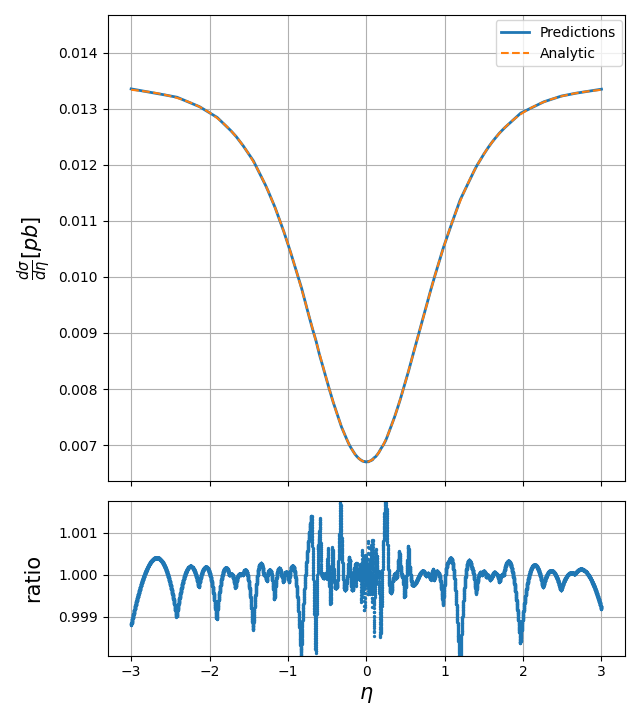
\includegraphics[width=8cm]{graphics/partonic_eta_model_eta_ratio}
	\caption{machine learning predictions vs analtisch berechnete Werte}
	\label{partonic_eta_model}
\end{figure}

\begin{figure}[tbp]
	\centering
	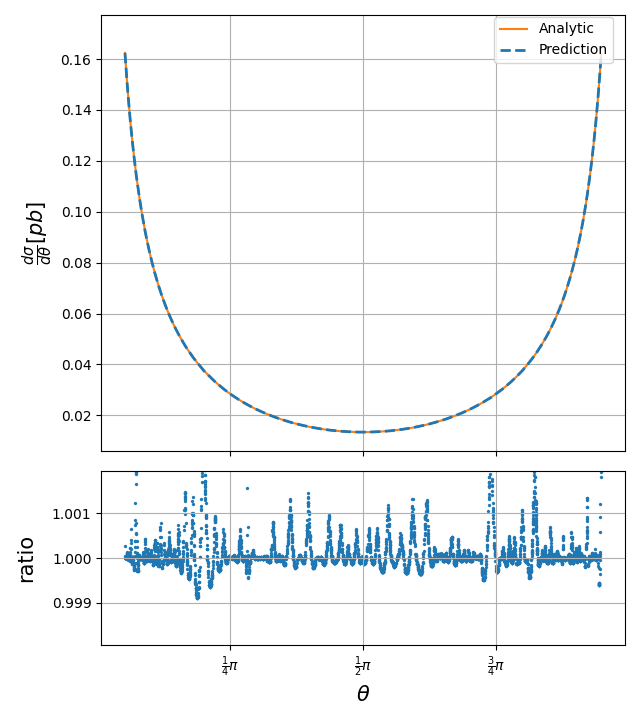
\includegraphics[width=8cm]{graphics/2}
	\caption{Predictions vs Analytisch auf relevantem Theta-Intervall}
\end{figure}

\begin{figure}[tbp]
	\centering
	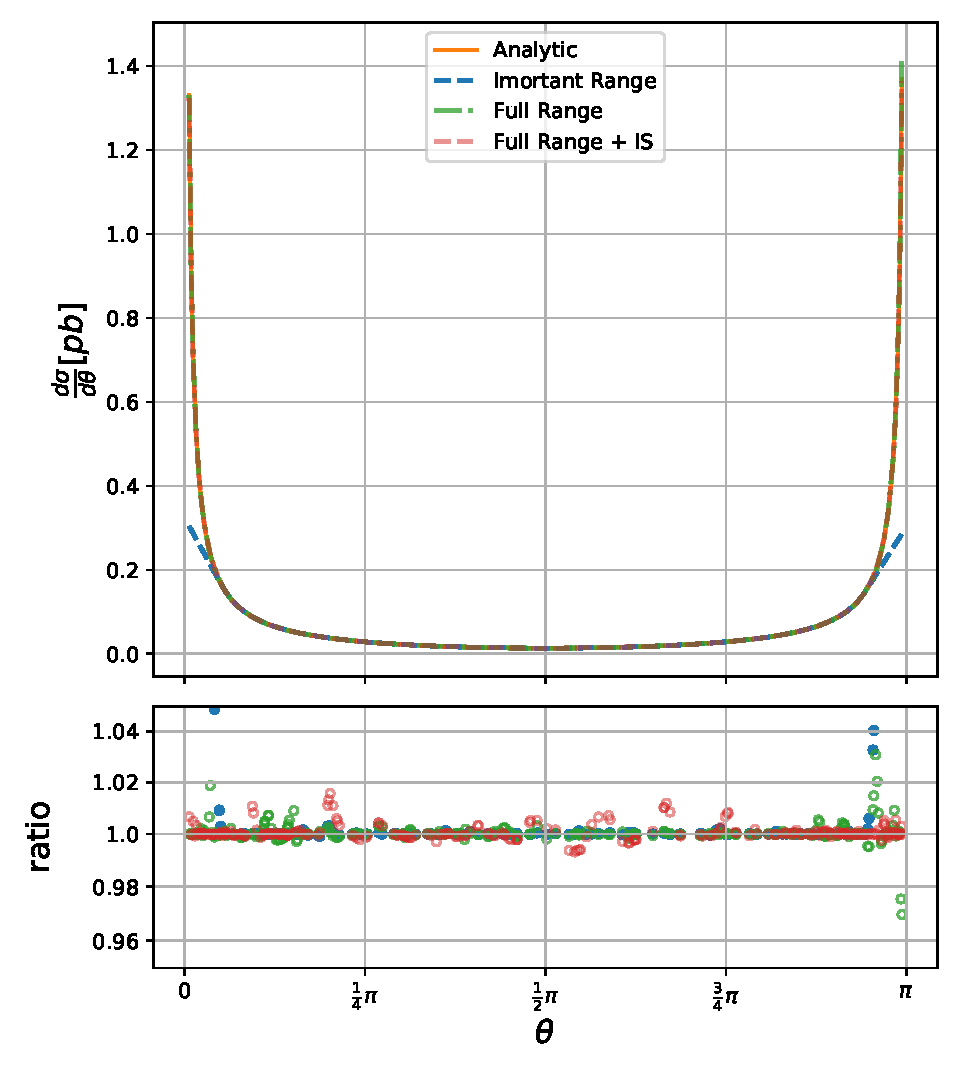
\includegraphics[width=9cm]{graphics/3}
	\caption{machine learning predictions vs analtisch berechnete Werte}
	\label{partonic_theta_model}
\end{figure}

\begin{figure}[tbp]
	\centering
	\subfloat[Modelle mit 60000 Traningspunkten]{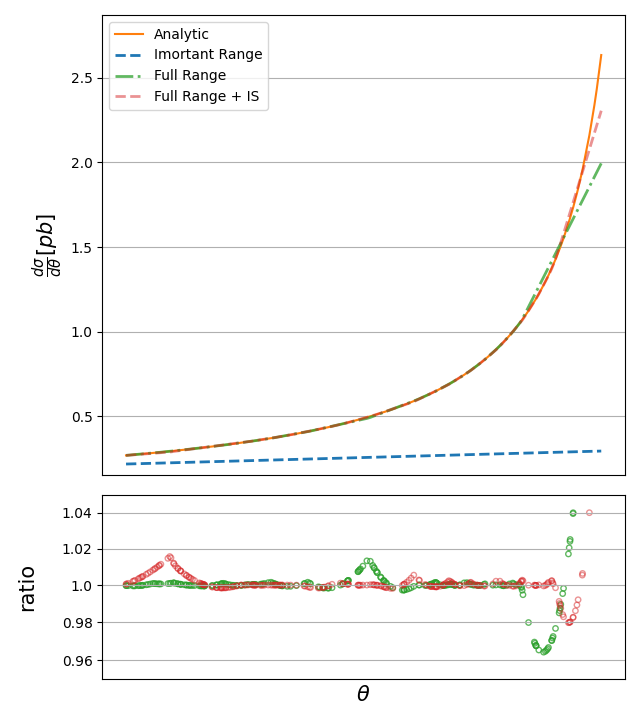
\includegraphics[width=7cm]{graphics/3.1}}
	\subfloat[Modelle mit 10000 Trainingspunkten]{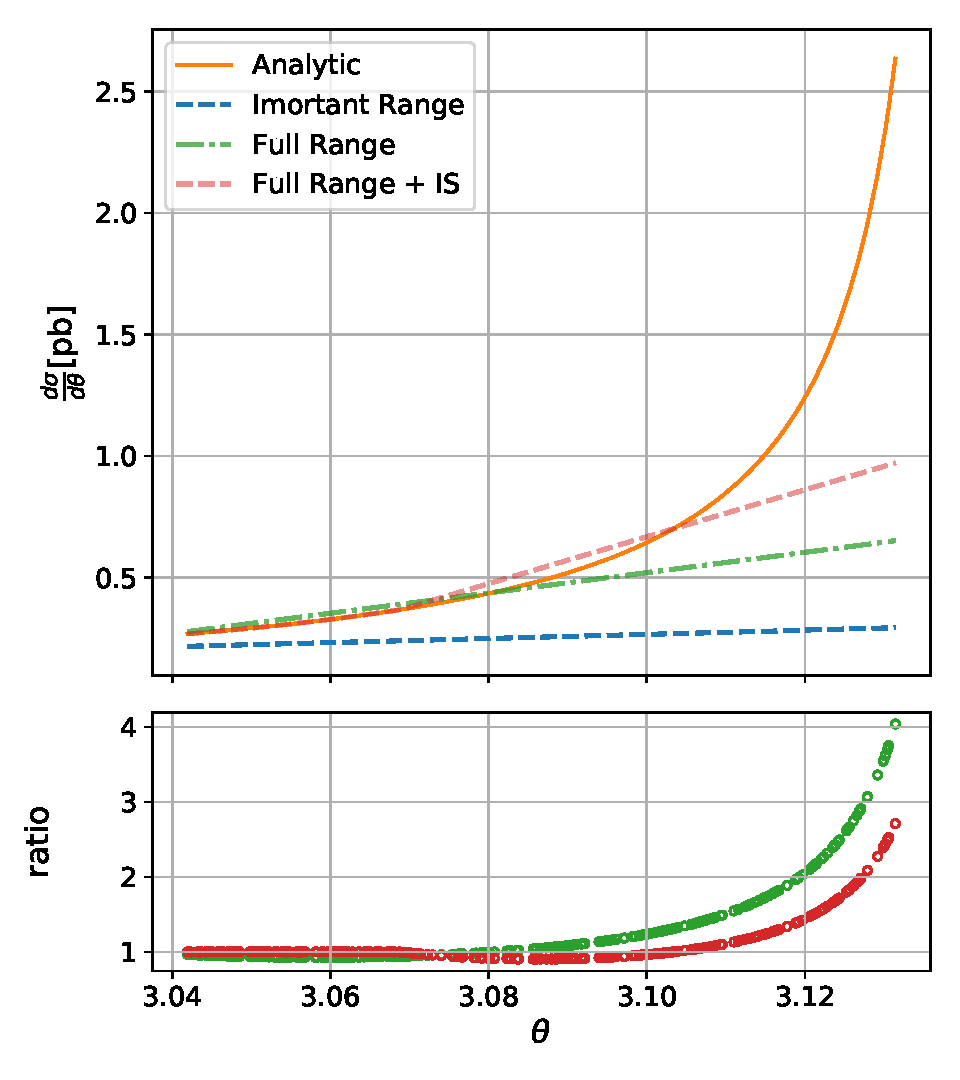
\includegraphics[width=7cm]{graphics/3.2}}
	\caption{Performance des Netzes für Randpunkte}
	\label{3.1 / 3.2}
\end{figure}

\begin{figure}
	\centering
	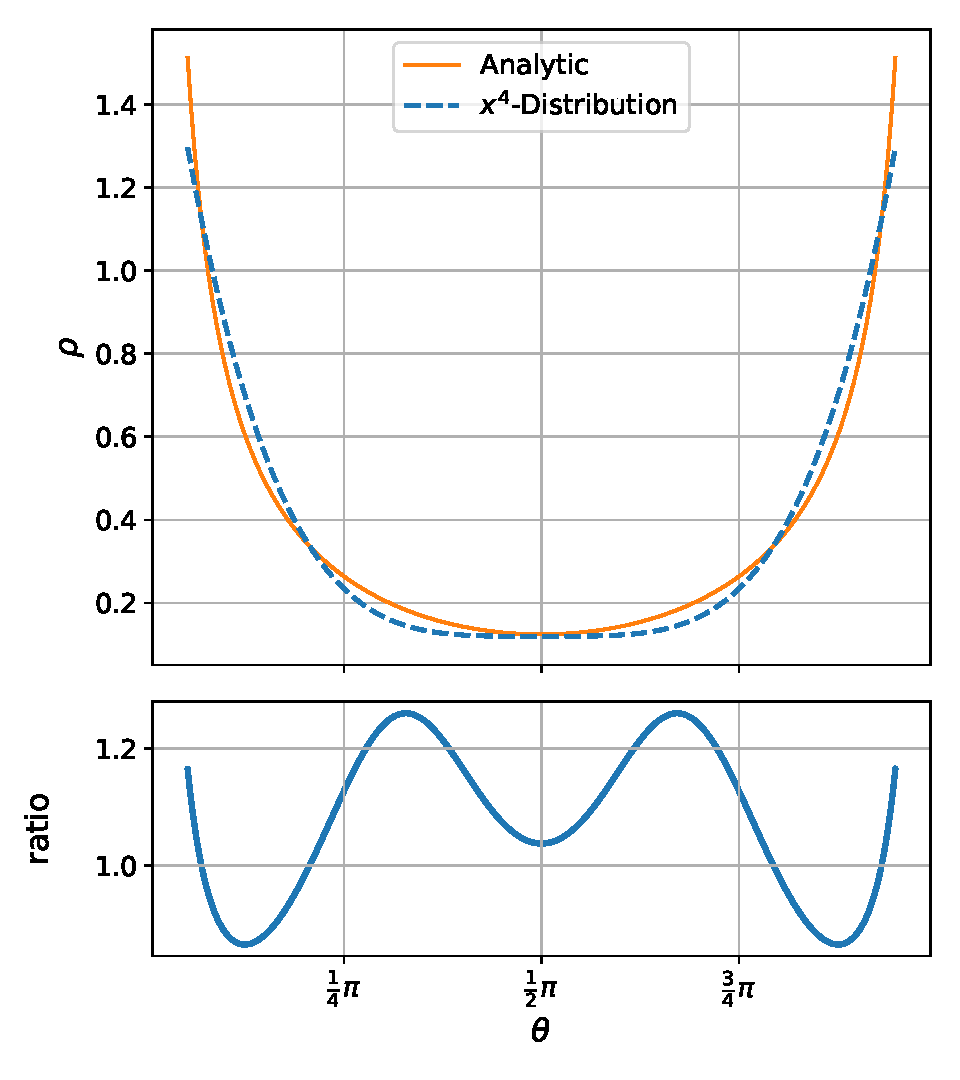
\includegraphics[width=8cm]{graphics/4}
	\caption{simples Importance Sampling, das die analytische Funktion annähern soll}
\end{figure}

\begin{figure}
	\centering
	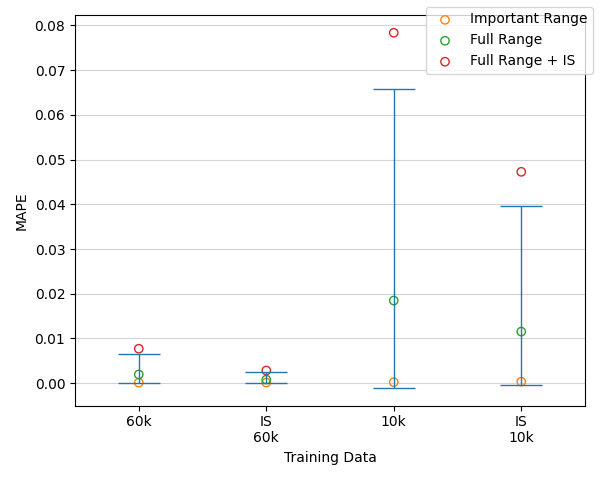
\includegraphics[width=9cm]{graphics/26}
	\caption{Vergleich der Performance von verschiedenen Theta-Modellen, die mit verschiedenen Datenmengen trainiert wurden. IS: Importance sampling. Auf der x-Achse sind die Trainings-Datenmengen und in der Legende die Test-Datenmengen}
\end{figure}

\section{Hadronischer Diphoton-Prozess}
\subsection{...}
% TODO Umrechnung in pb für Grafik 8
\begin{figure}[tbp]
	\centering
	\subfloat[]{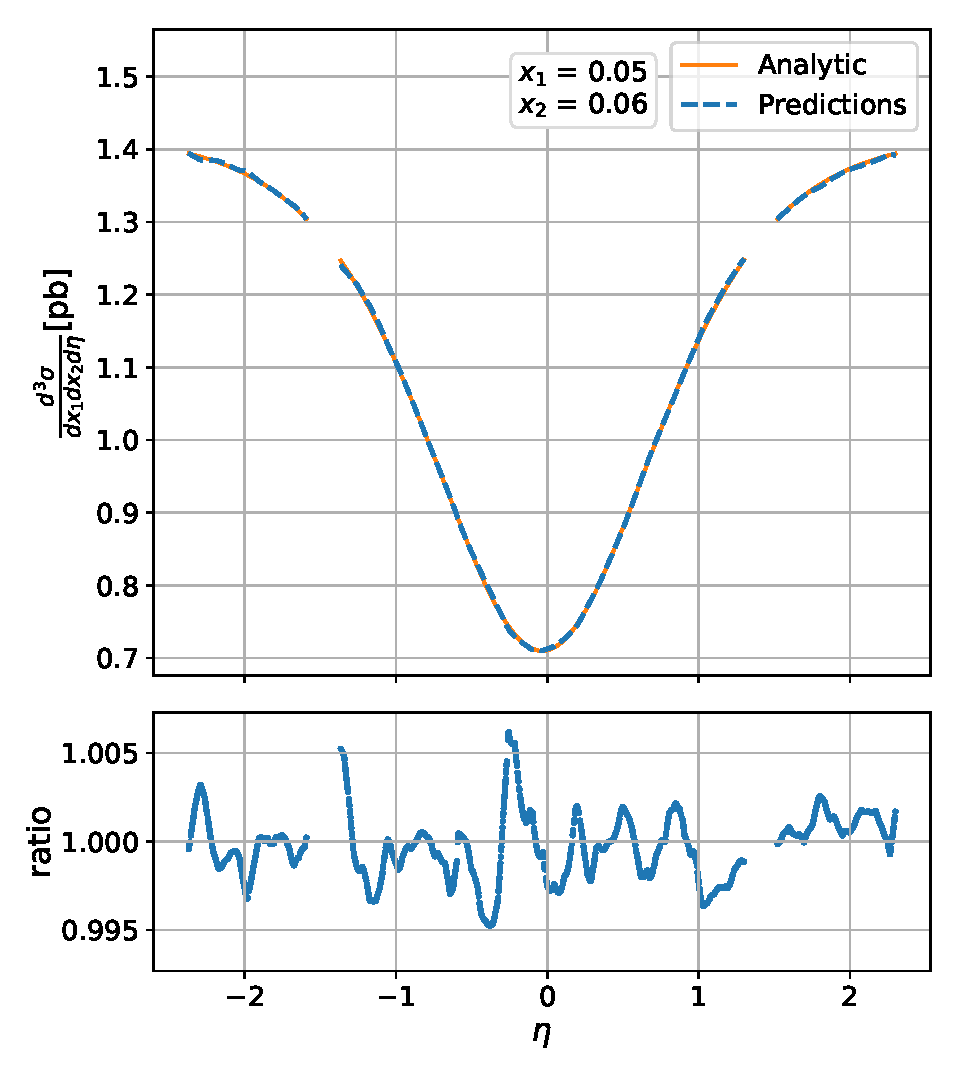
\includegraphics[width=7cm]{graphics/5}}
	\subfloat[]{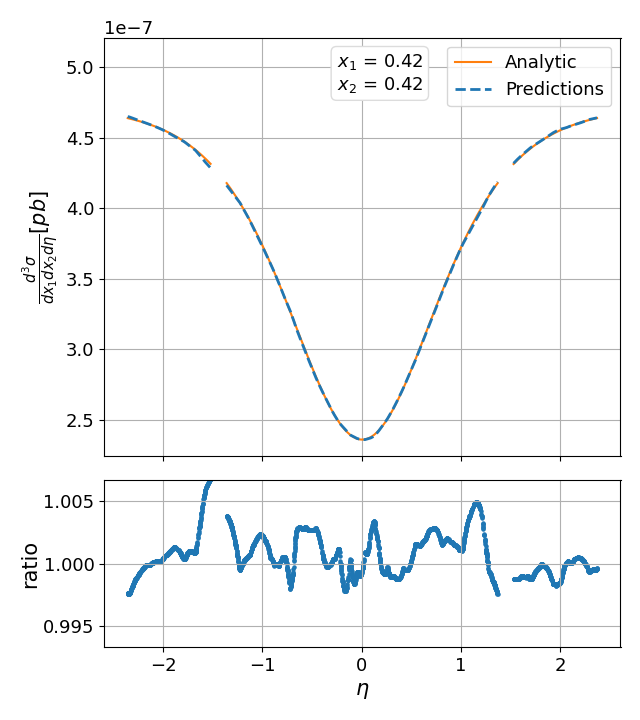
\includegraphics[width=7cm]{graphics/8}}
	\caption{Schnitte des differentiellen Wirkungsquerschnitts in $\eta$}
	\label{5,8}
\end{figure}

\begin{figure}[tbp]
	\centering
	\subfloat[]{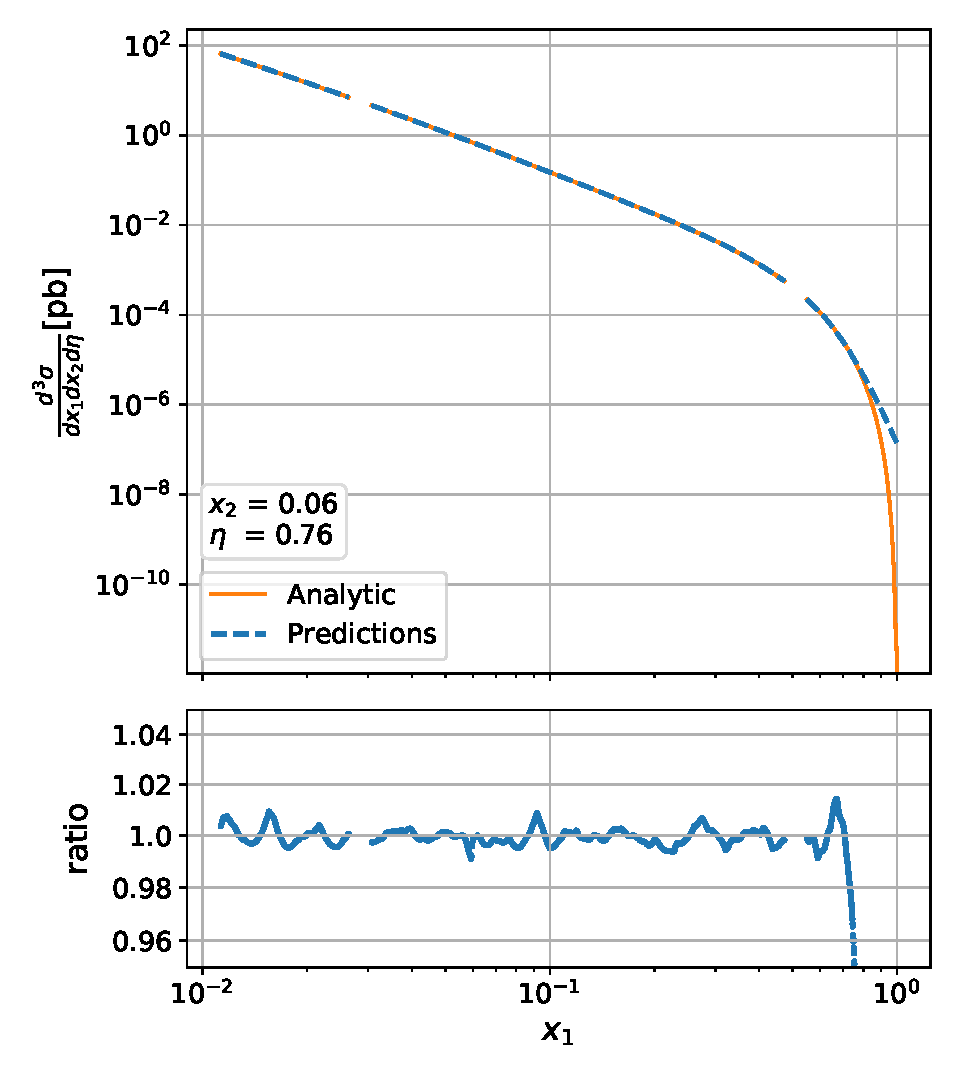
\includegraphics[width=7cm]{graphics/6}}
	\subfloat[]{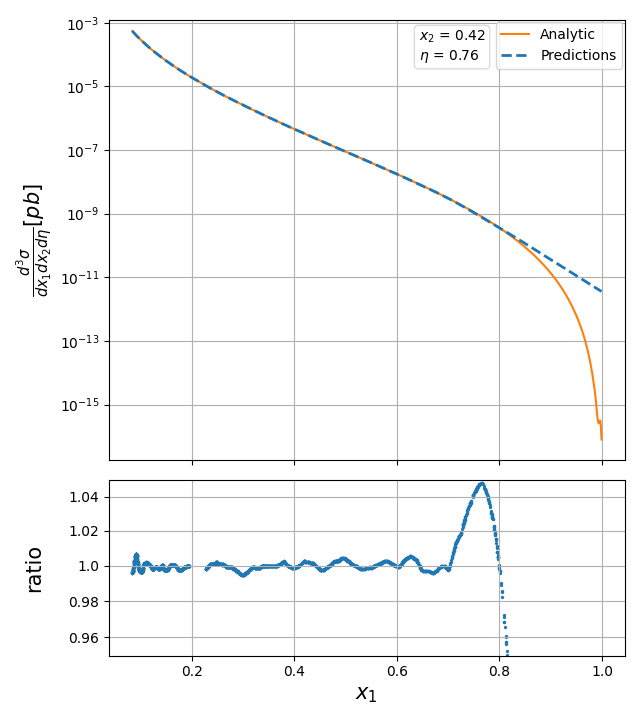
\includegraphics[width=7cm]{graphics/9}}
	\caption{Schnitte des differentiellen Wirkungsquerschnitts in $x_1$}
	\label{6,9}
\end{figure}

\begin{figure}[tbp]
	\centering
	\subfloat[]{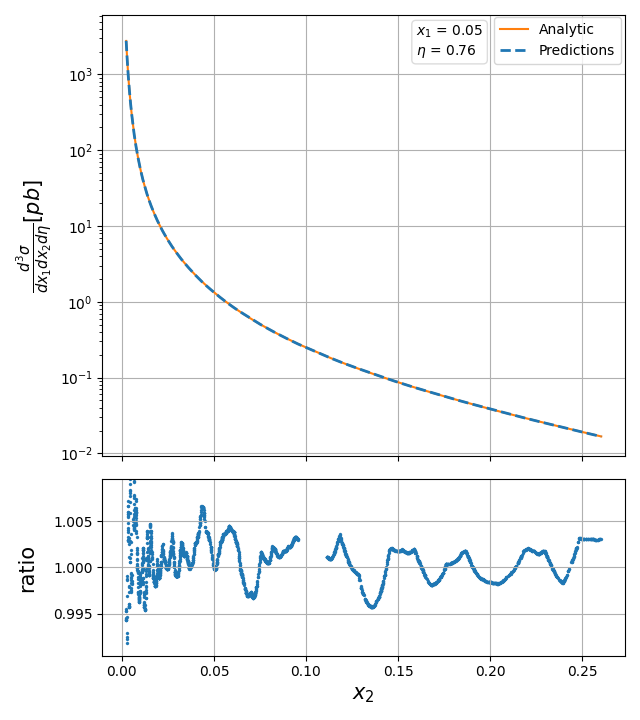
\includegraphics[width=7cm]{graphics/7}}
	\subfloat[]{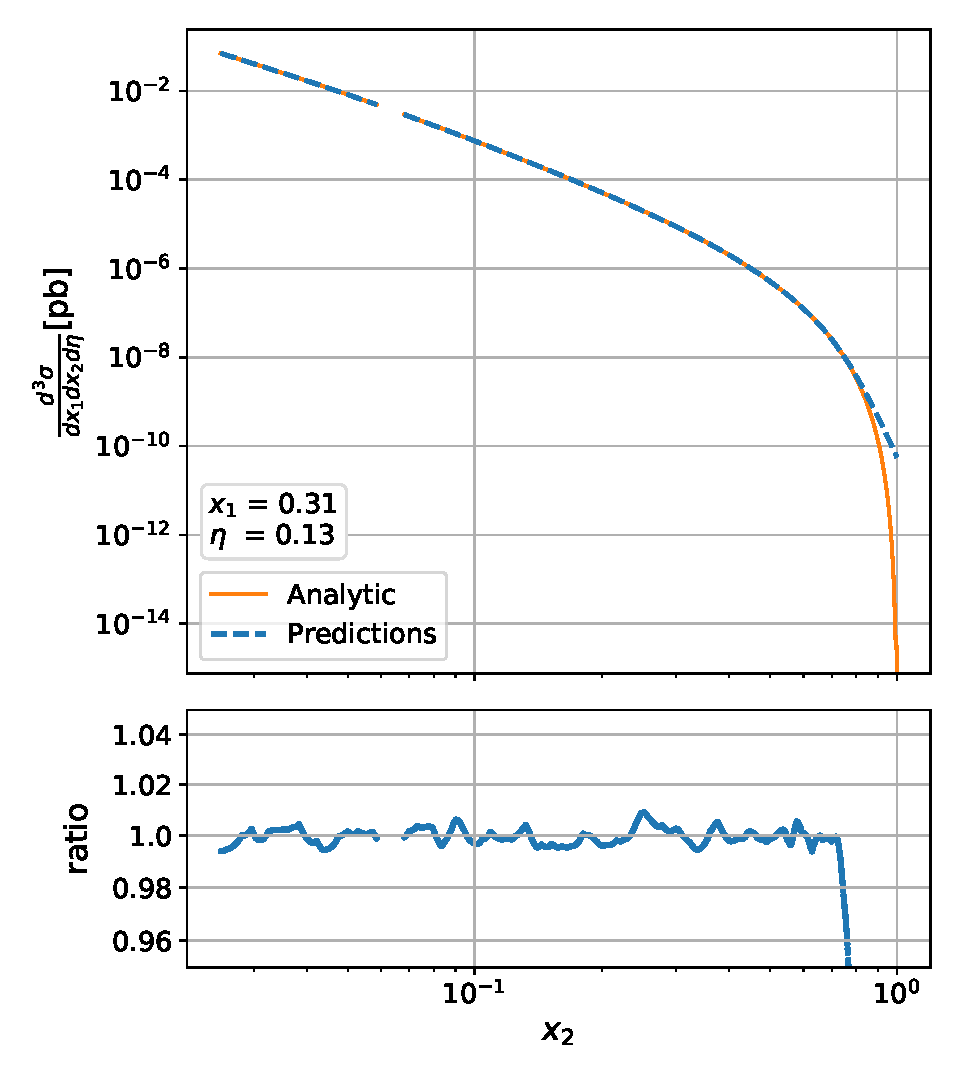
\includegraphics[width=7cm]{graphics/10}}
	\caption{Schnitte des differentiellen Wirkungsquerschnitts in $x_2$}
	\label{7,10}
\end{figure}
\subsection{Vergleiche}
\begin{figure}[tbp]
	\centering
	\subfloat[Vergleich für verschiedene Loss-Funktionen]{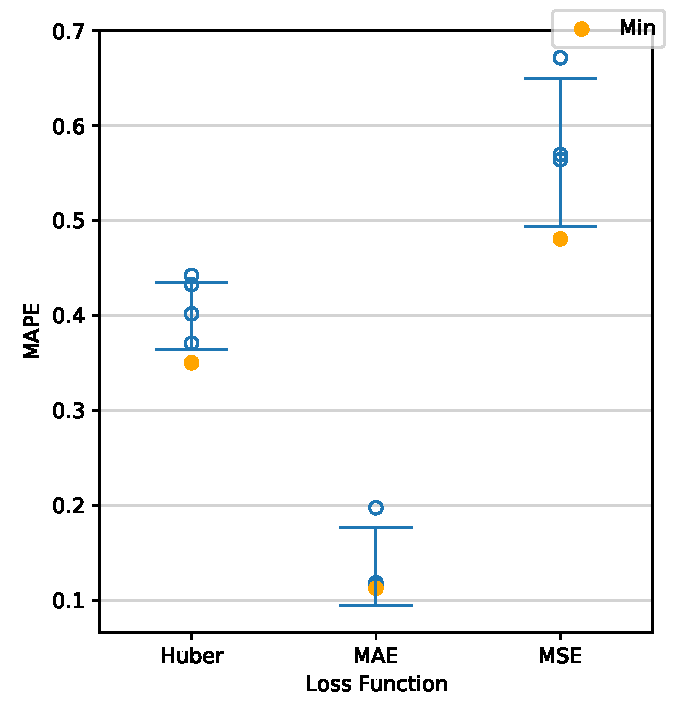
\includegraphics[width=7cm]{graphics/12}}
	\subfloat[Vergleich für verschiedene Optimizer]{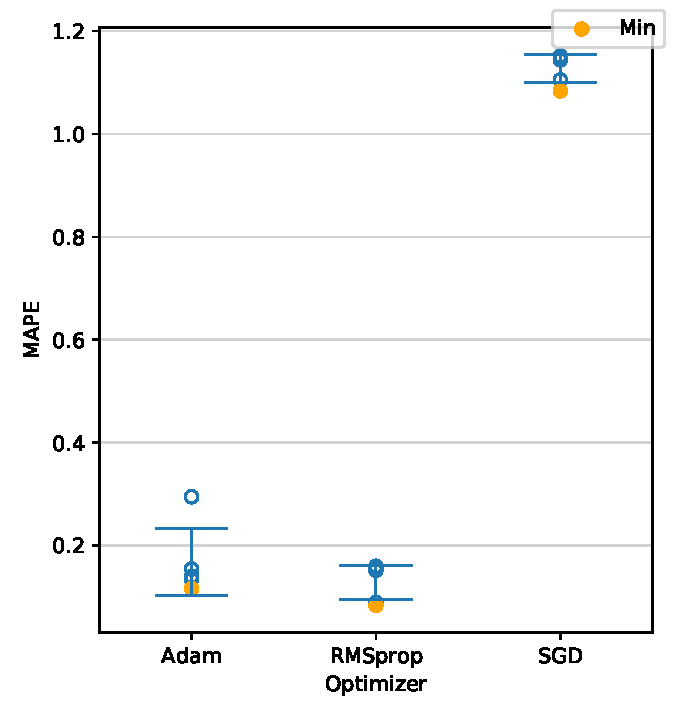
\includegraphics[width=7cm]{graphics/13}} \\
	\subfloat[Vergleich für verschiedene Anzahl an Trainigspunkten]{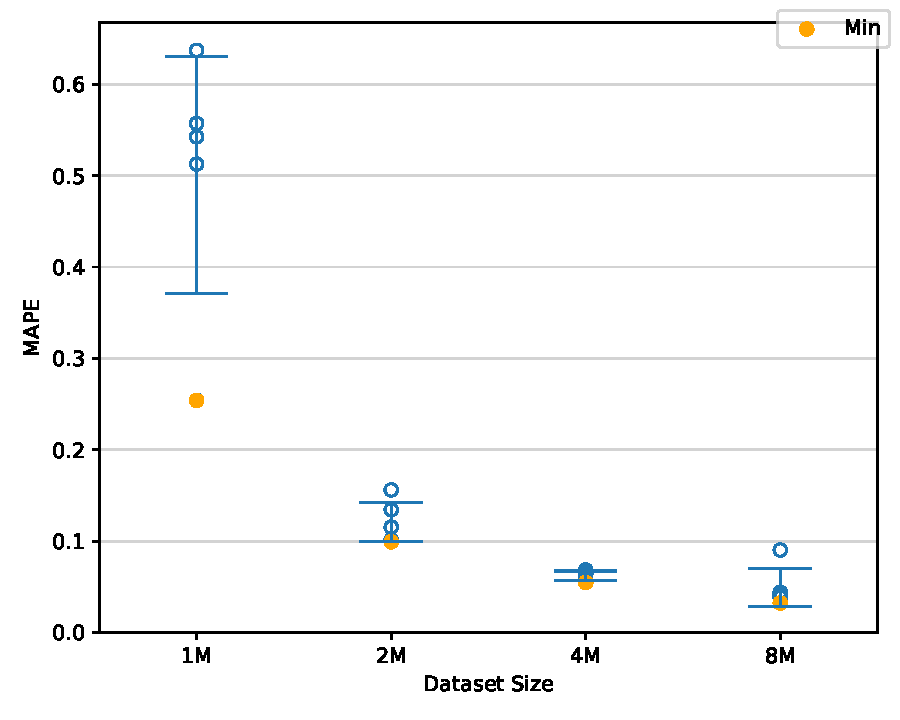
\includegraphics[width=7cm]{graphics/16}}
	\subfloat[Vergleich für verschiedene Anfangs-Lernraten]{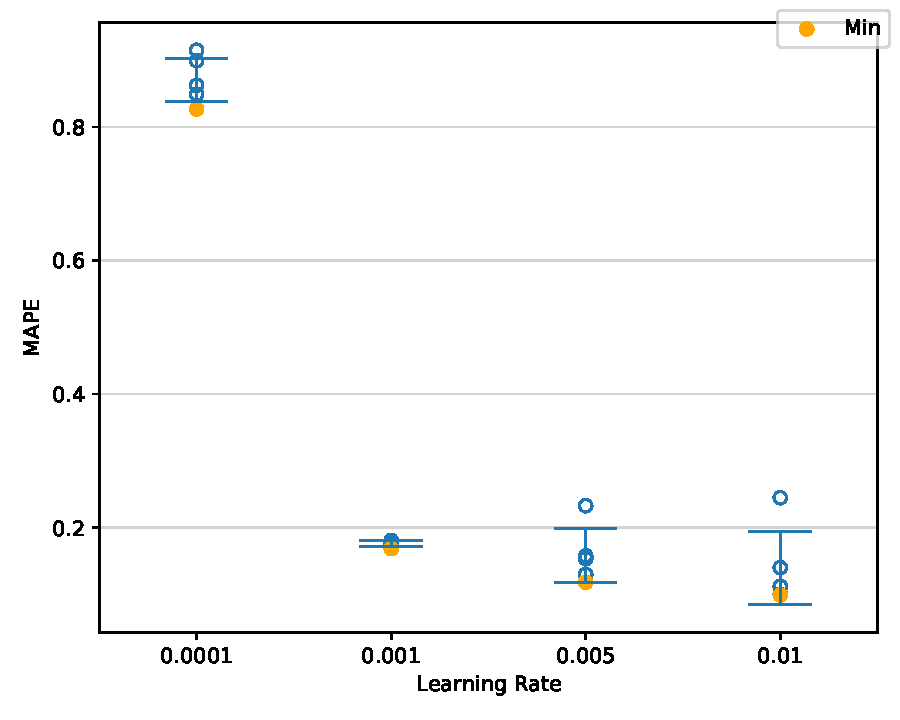
\includegraphics[width=7cm]{graphics/36}}
	\caption{Vergleich von Hyperparametern (I), MAPE: Mean-Absolute-Percentage-Error}
	\label{12,13,16,36}
\end{figure}

\begin{figure}[tbp]
	\centering
	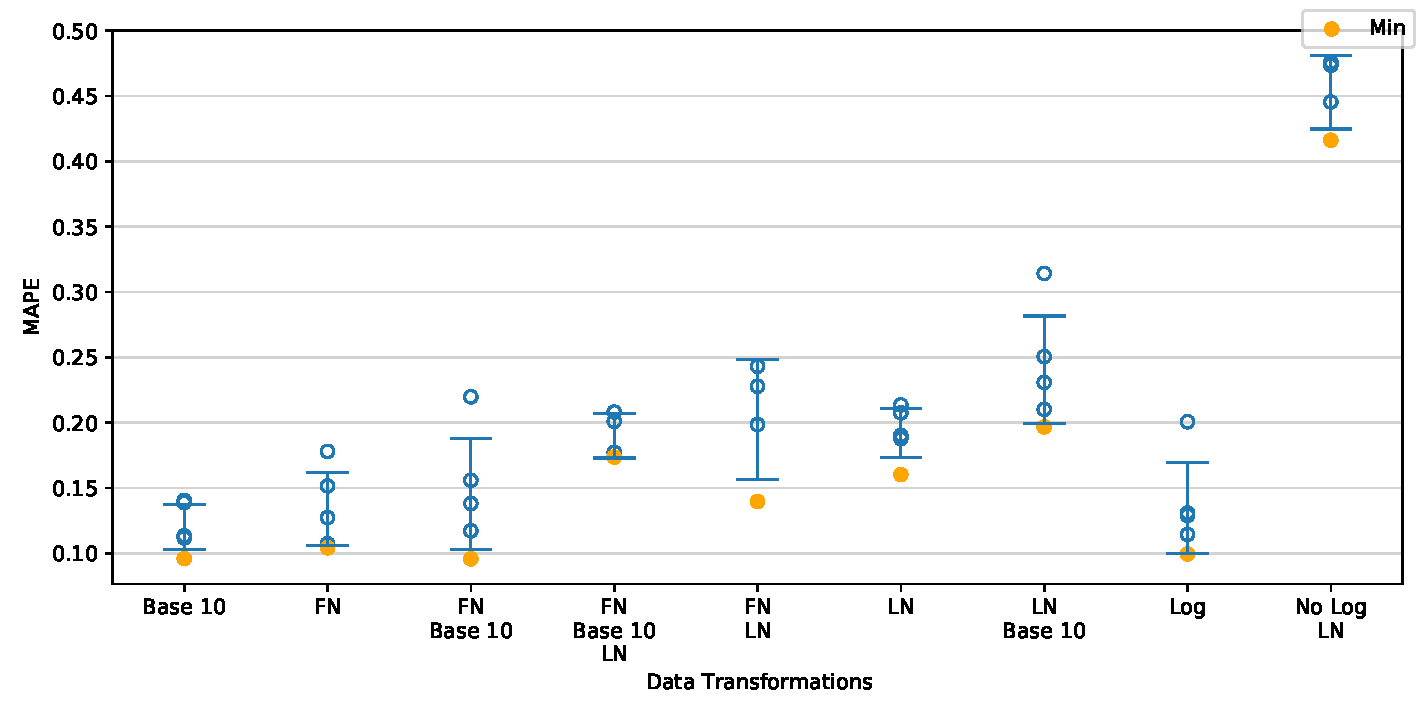
\includegraphics[width=14cm]{graphics/17,18}
	\caption{wichtig: die Daten-Transformationen ohne die überhaupt nichts geht \newline
			Base 10: Daten werden mit Logarithmus zur Basis 10 transformiert \newline
			FN: Feature-Normalization \newline
			LN: Label-Normalization \newline
			Log: Nur Scaling+Logarithmus \newline 
			No Log: Nur Scaling}
\end{figure}
\begin{figure}[tbp]
	\centering
	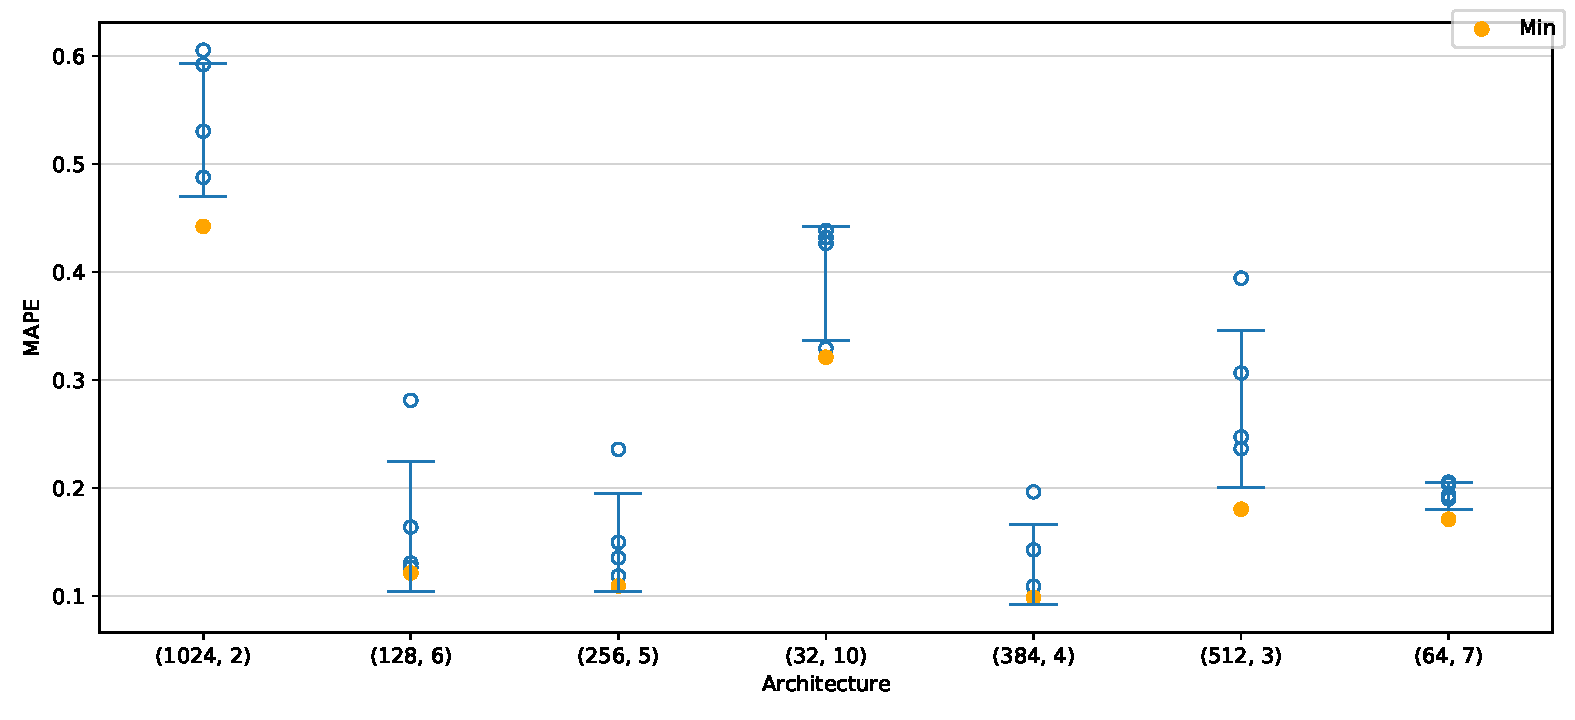
\includegraphics[width=14cm]{graphics/33}
	\caption{Vergleich für verschiedene Modell-Architekturen. \newline
		x-Labels in (Units, Nr of Layers)}
\end{figure}

\begin{figure}[tbp]
	\centering
	\subfloat[Vergleich für verschiedene Zahlen an Layern]{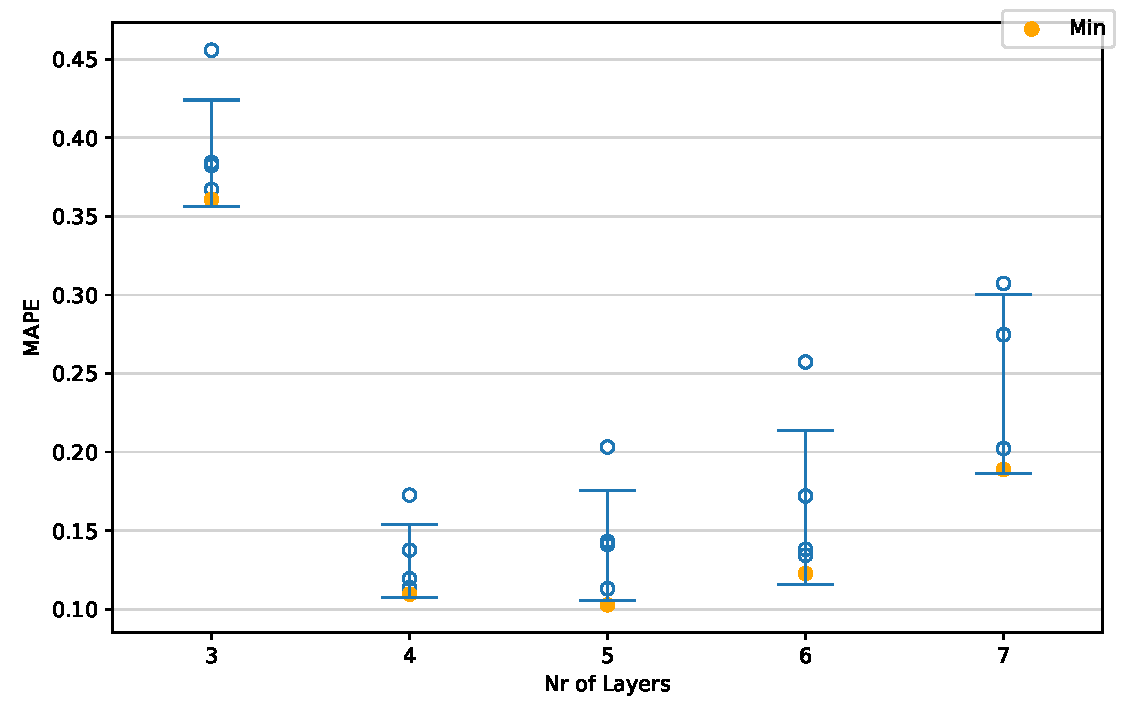
\includegraphics[width=7cm]{graphics/14}}
	\subfloat[Vergleich für verschiedene Zahlen an Units]{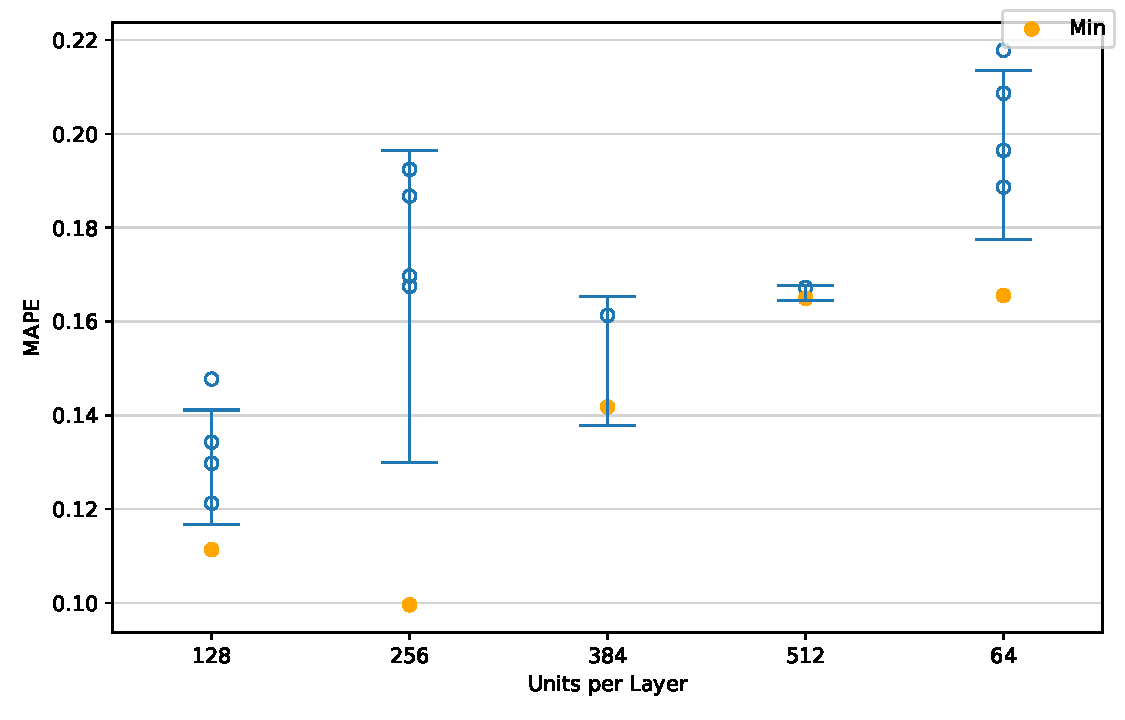
\includegraphics[width=7cm]{graphics/15}} \\
	\subfloat[Vergleich für verschiedene Activation-Functions]{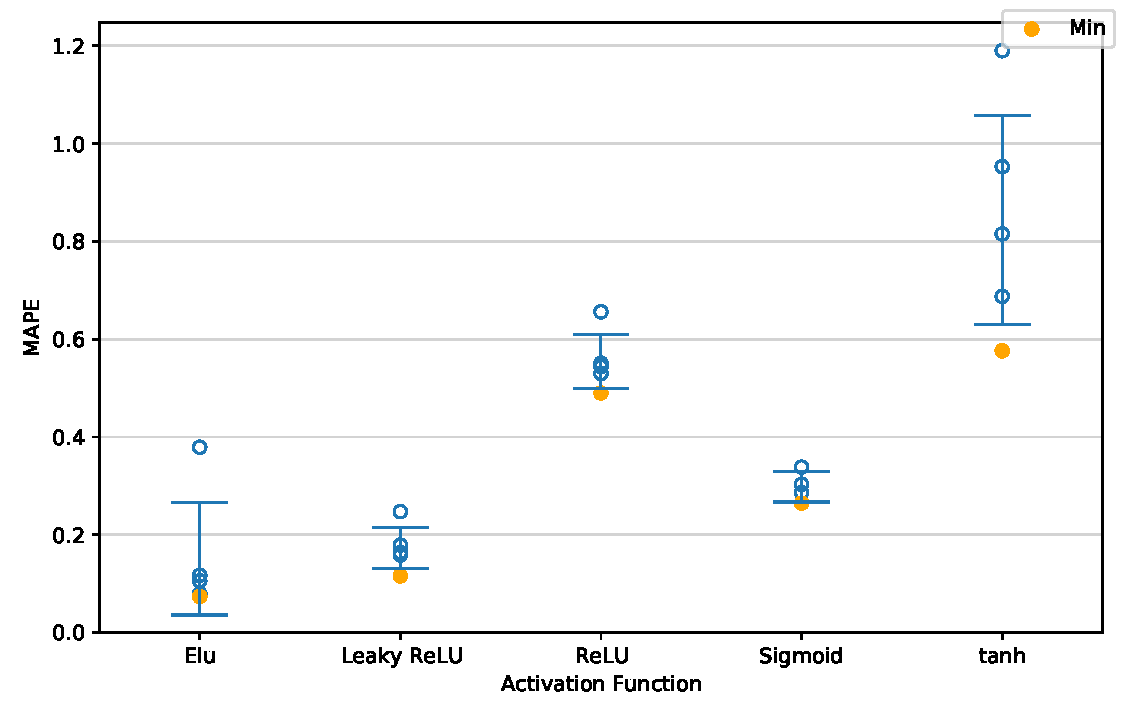
\includegraphics[width=7cm]{graphics/19}}
	\subfloat[Vergleich für verschiedene Batch-Sizes]{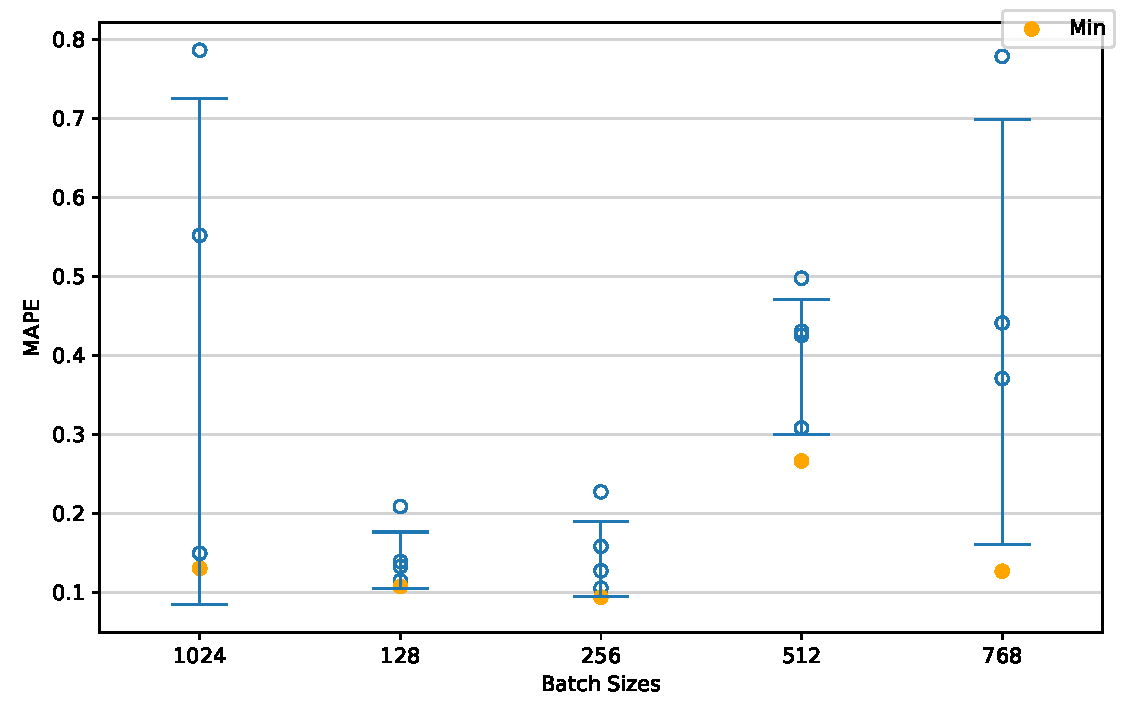
\includegraphics[width=7cm]{graphics/20}}
	\caption{Vergleich von Hyperparametern (II), MAPE: Mean-Absolute-Percentage-Error}
	\label{14,15,19,20}
\end{figure}


\section{Reweweight zwischen Fits der Partondichtefunktionen}
\subsection{...}

\begin{figure}[tbp]
	\centering
	\subfloat[Schnitt in $x_1$]{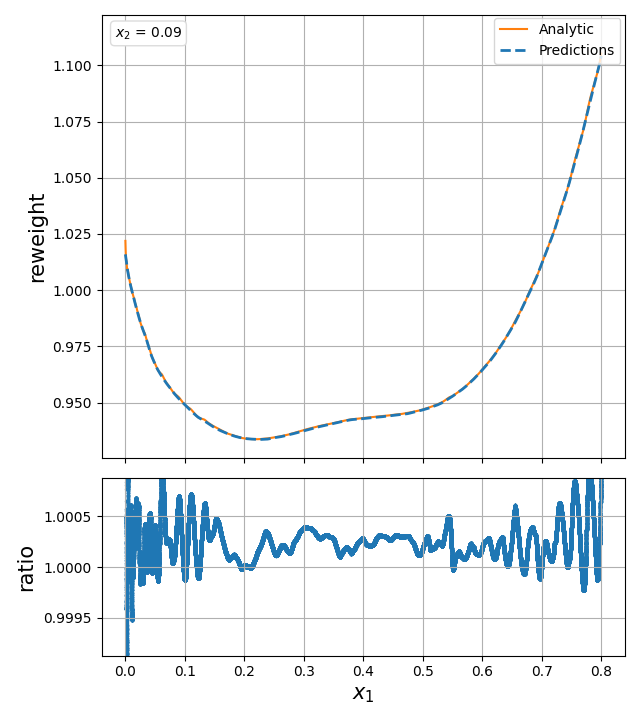
\includegraphics[width=7cm]{graphics/32}}
	\subfloat[Schnitt in $x_2$]{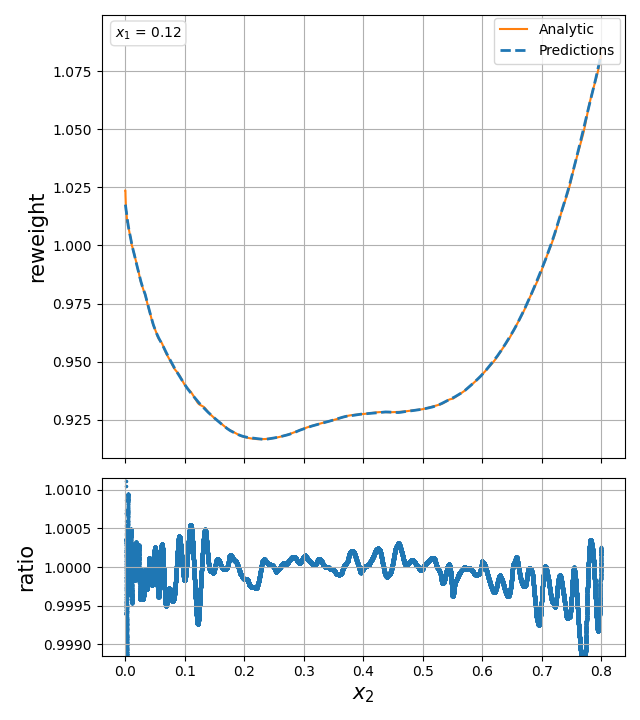
\includegraphics[width=7cm]{graphics/33_1}} 
	\caption{Vlt noch 2 3D-plots, einmal die analytischen Reweights, gelernte Reweights werden aber gleich aussehen bei der geringen abweichung}
	\label{32,33}
\end{figure}
\begin{figure}[tbp]
	\centering
	\subfloat[Schnitt in $x_1$]{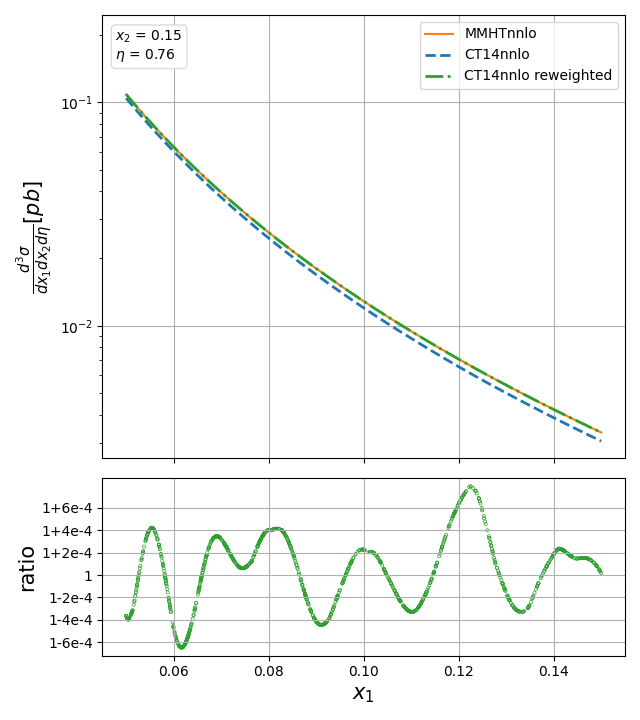
\includegraphics[width=7cm]{graphics/22.0}} 
	\subfloat[Schnitt in $x_2$]{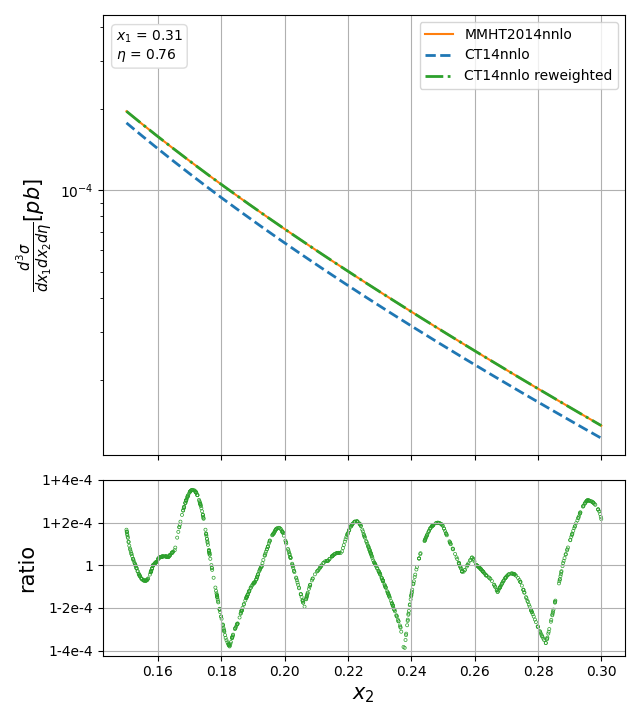
\includegraphics[width=7cm]{graphics/23.1}} \\
	\subfloat[Schnitt in $\eta$]{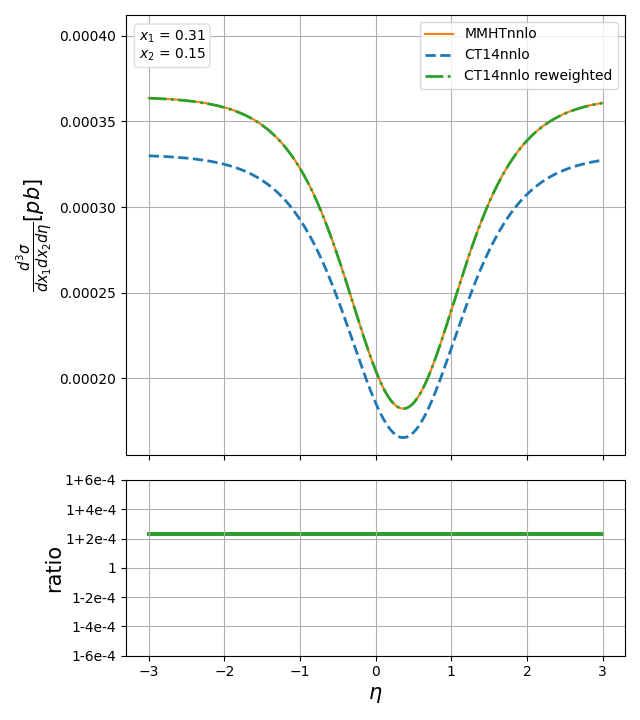
\includegraphics[width=7cm]{graphics/21.0}}
	\caption{Reweight von CT14nnlo auf MMHT2014nnlo mittels gelernten Weigths}
	\label{21,22,23}
\end{figure}

\begin{figure}
	\centering
	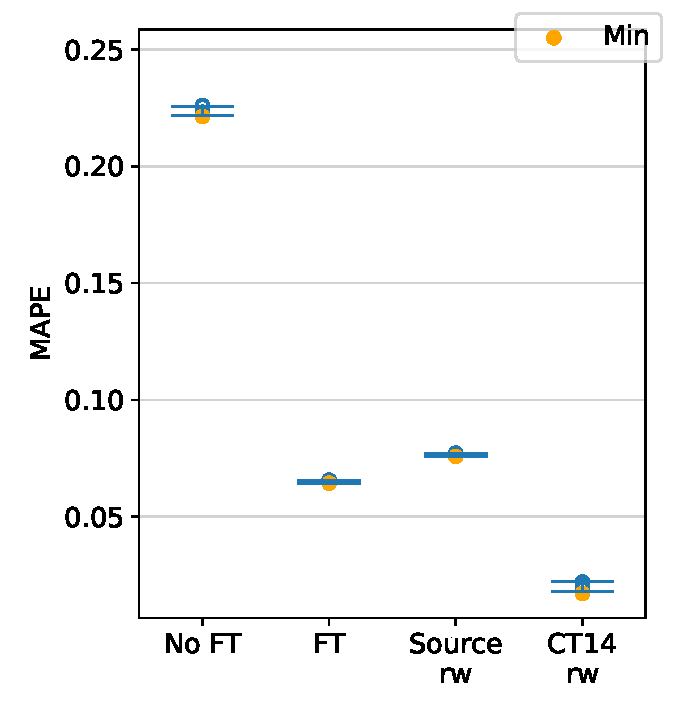
\includegraphics[width=6cm]{graphics/25,29}
	\caption{Vergleich von Transfer Learning mit und ohne Fine-Tuning, Vergleich mit gereweithenem source model kommt noch}
\end{figure}



\section{Transfer-Learning zwischen verschiedenen Fits der Partondichtefunktionen}
\subsection{...}
\begin{figure}[tbp]
	\centering
	\subfloat[Schnitt in $x_1$]{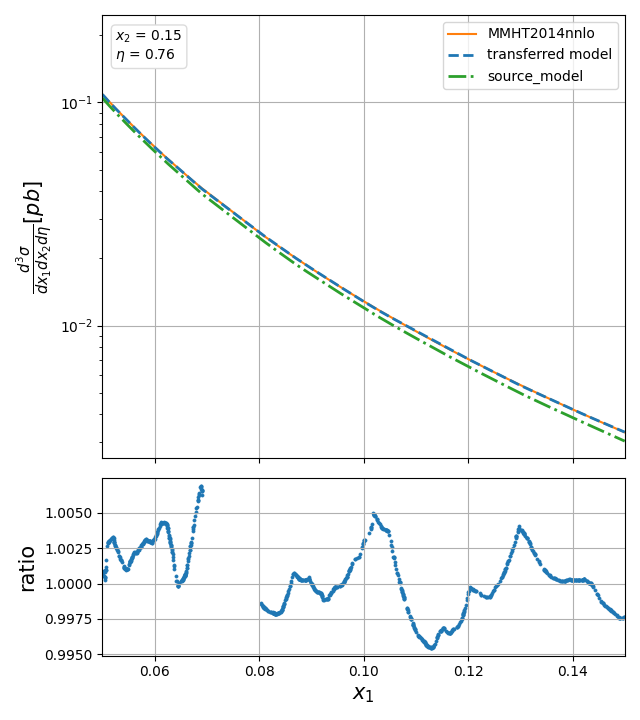
\includegraphics[width=7cm]{graphics/34.0}} 
	\subfloat[Schnitt in $x_2$]{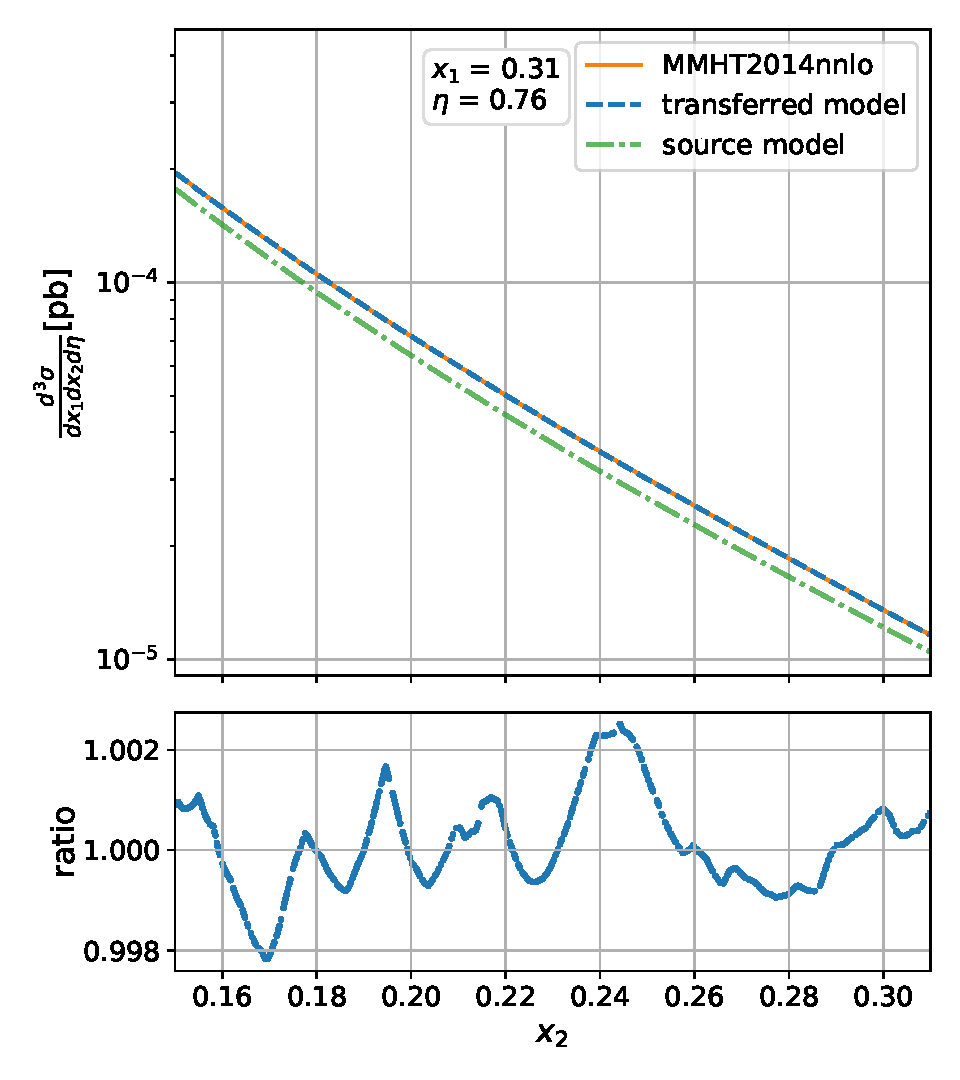
\includegraphics[width=7cm]{graphics/35.1}} \\
	\subfloat[Schnitt in $\eta$]{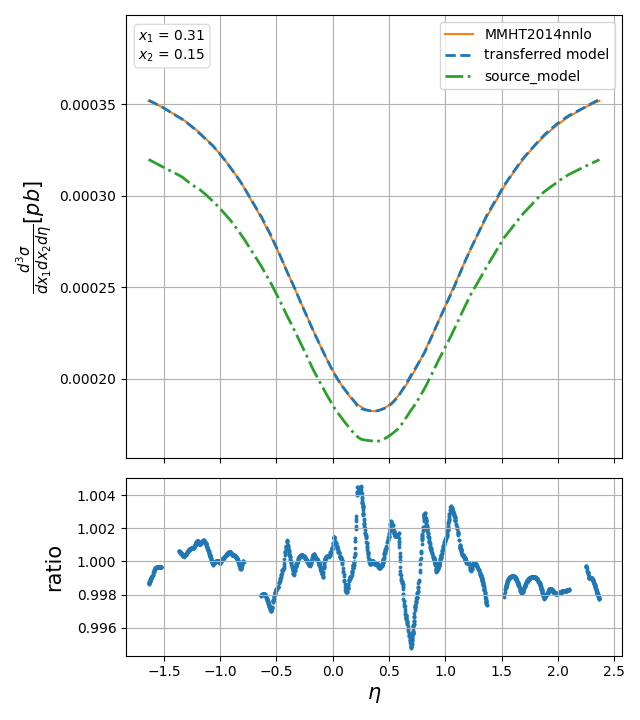
\includegraphics[width=7cm]{graphics/24}}
	\caption{Transferiertes Model von Source Model zum Transfer model}
	\label{34,35,24}
\end{figure}

\begin{figure}[tbp]
	\centering
	\subfloat[Schnitt in $x_1$]{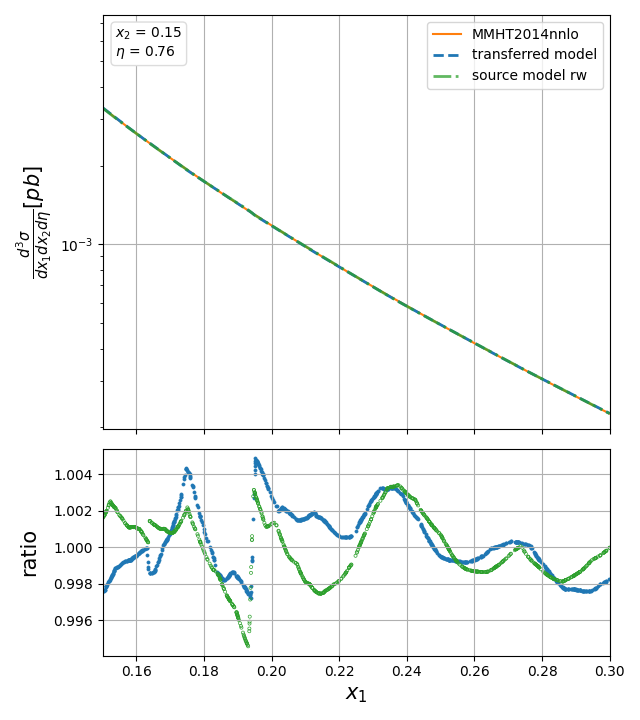
\includegraphics[width=7cm]{graphics/34.2}} 
	\subfloat[Schnitt in $x_2$]{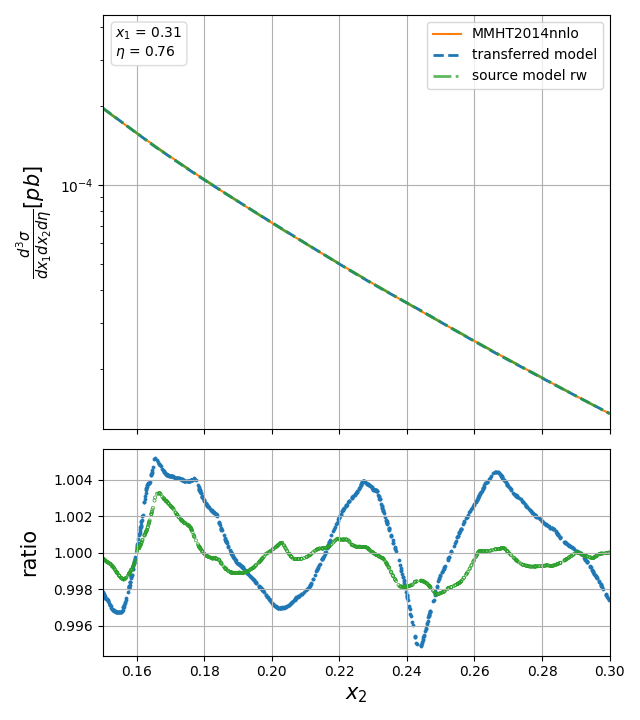
\includegraphics[width=7cm]{graphics/35.2}} \\
	\subfloat[Schnitt in $\eta$]{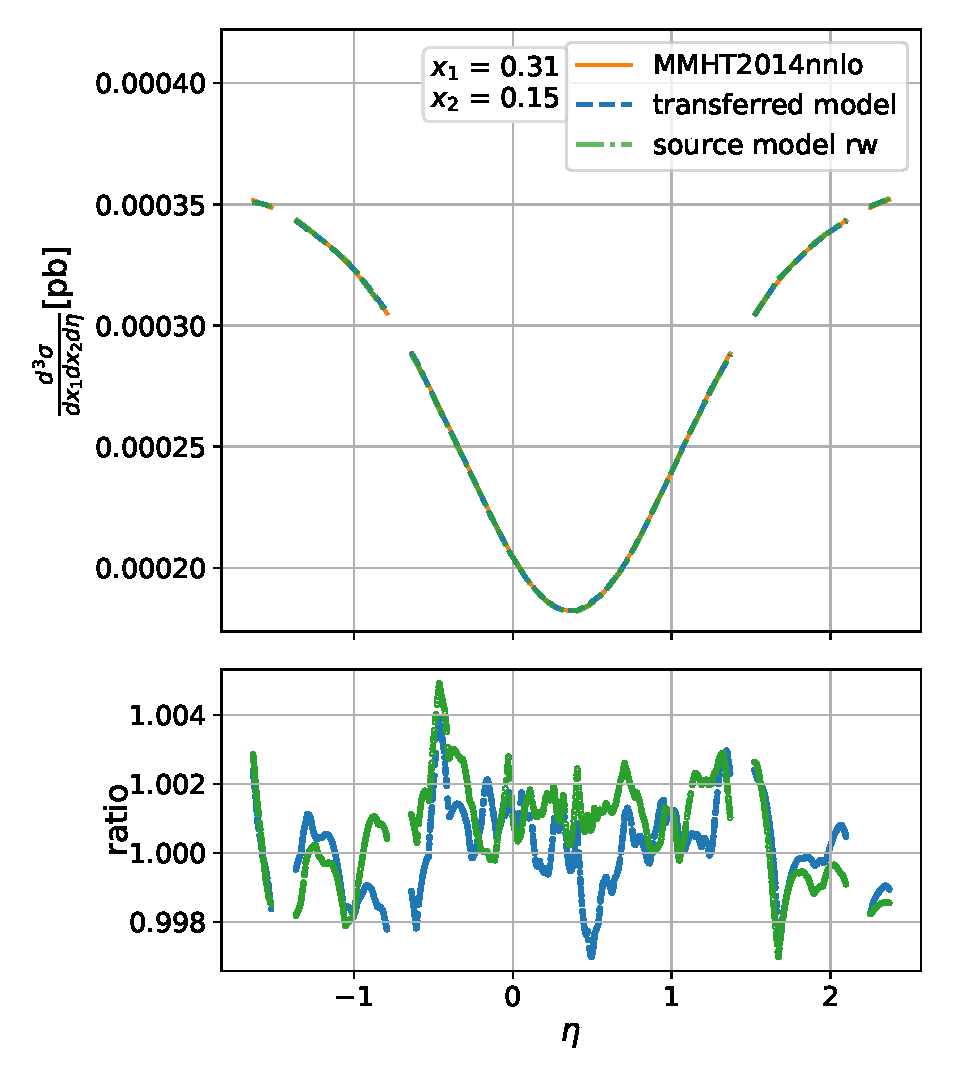
\includegraphics[width=7cm]{graphics/24.2}}
	\caption{Vergleich transferiertes Modell, gereweightetes Source Model \newline
		rw: reweighted}
	\label{34,35,24,reweight}
\end{figure}


\begin{figure}[tbp]
	\centering
	\subfloat[]{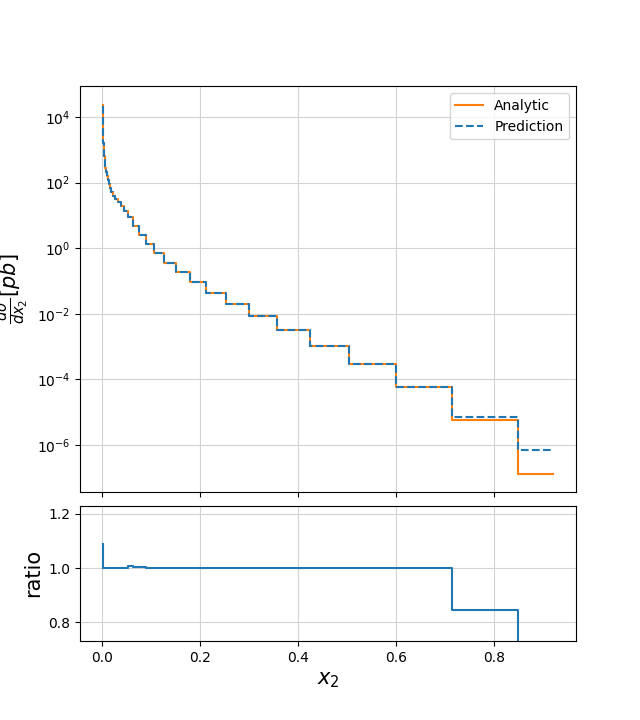
\includegraphics[width=7cm]{graphics/27}} 
	\subfloat[]{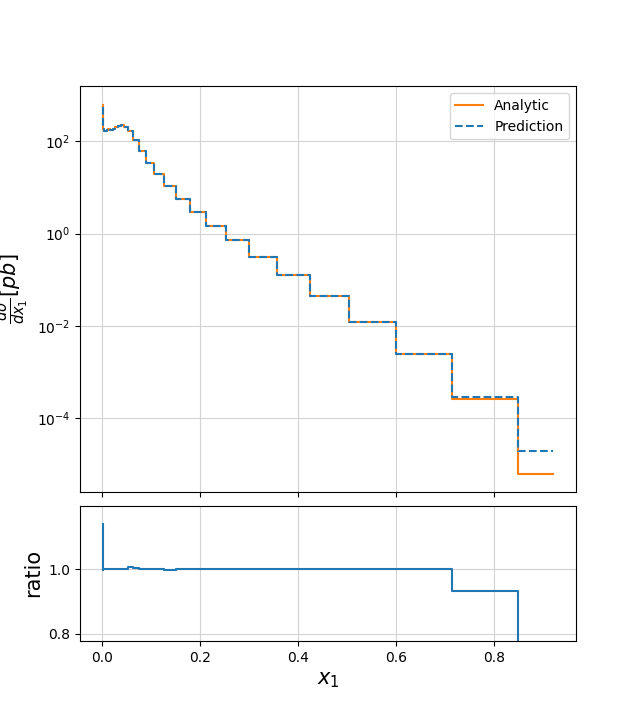
\includegraphics[width=7cm]{graphics/28}} \\
	\subfloat[]{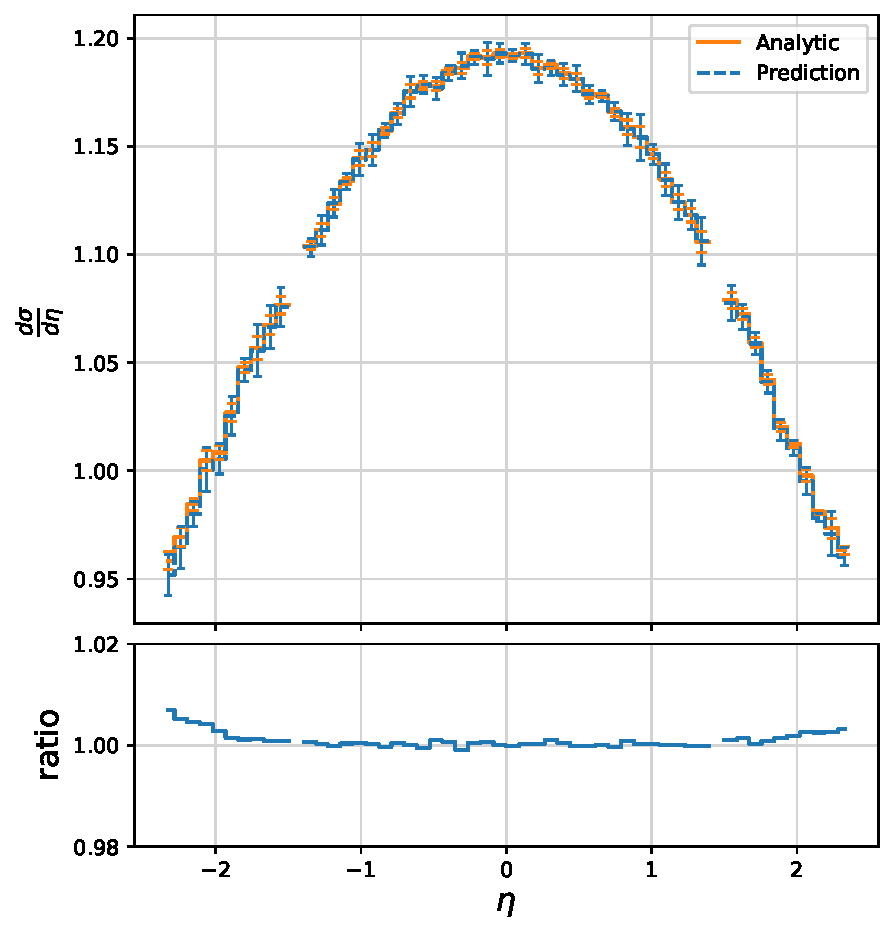
\includegraphics[width=7cm]{graphics/11}}
	\caption{MC-Integrationen über zwei Freiheitsgrade}
	\label{11,27,28}
\end{figure}

\chapter{Zusammenfassung und Diskussion}
\section{Zusammenfassung}
\section{Diskussion}
\section{Ausblick}


\appendix
\chapter{Anhang}
\begin{table}
	\centering
	\begin{tabular}{|l|l|}
		\hline
		Callback & Config \\
		\hline
		\multirow{3}{*}{LearningRateScheduler} & nach einem Offset von 10 Epochen, wird die \\
		& Learning-Rate nach jeder Epoche um $5\%$ reduziert, \\
		& bis diese auf $5 \cdot 10^{-8}$ abgefallen ist. \\
		\hline
		\multirow{2}{*}{ReduceLROnPlateau}& Fällt der Loss nach einer Epoche nicht um mindestens\\
		& $2 \cdot 10^{-6}$, wird die Learning-Rate um $50\%$ reduziert.\\
		\hline
		\multirow{2}{*}{EarlyStopping}& Fällt der Loss in drei aufeinanderfolgenden Epochen nicht um  \\ 
		& mindestens $2 \cdot 10^{-7}$ ab, wird der Trainingsvorgang gestoppt.\\
		\hline
	\end{tabular}
	\label{callbacks}
\end{table}
\section{Grafiken}
\section{Source-Code}

%--------------------------------------------------------------------
% Vorlage für eine Abschlussarbeit
% Darf ohne Einschränkungen weiterverwendet und abgeändert werden.
% mehr zur Verwedung in der README.md
% ⓒ (CC0) 2016, 2018 Henning Iseke <h_i_@online.de>
%--------------------------------------------------------------------

\printbibliography
\cleardoublepage
\pagestyle{empty}
\section*{Danksagung} % TODO: anpassen
Danke an Christial Wiel.
\cleardoublepage
%TODO: anpassen
\section*{Erklärung}
Hiermit erkläre ich, dass ich die vorliegende Arbeit im Rahmen der Betreuung am
\institut{} ohne unzulässige Hilfe Dritter verfasst habe und alle verwendeten
Quellen als solche gekennzeichnet habe.

% Zur Beschriftung
\vspace{5\baselineskip}
\noindent
\rule[0.5ex]{20em}{0.5pt}\rule[0.5ex]{10em}{0.5pt}\\
Ort, Datum\hspace{8em}Unterschrift 

%
%--------------------------------------------------------------------
% Vorlage für eine Abschlussarbeit
% Darf ohne Einschränkungen weiterverwendet und abgeändert werden.
% mehr zur Verwedung in der README.md
% ⓒ (CC0) 2016, 2018 Henning Iseke <h_i_@online.de>
%--------------------------------------------------------------------

\printbibliography
\cleardoublepage
\pagestyle{empty}
\section*{Acknowledgements} % TODO: anpassen, britsh english
<Thank you>
\cleardoublepage
\begin{german}
\section*{Erklärung} 
%TODO: anpassen
Hiermit erkläre ich, dass ich die vorliegende Arbeit im Rahmen der Betreuung am
\institut{} ohne unzulässige Hilfe Dritter verfasst habe und alle verwendeten
Quellen als solche gekennzeichnet habe.

% Zur Beschriftung
\vspace{5\baselineskip}
\noindent
\rule[0.5ex]{20em}{0.5pt}\rule[0.5ex]{10em}{0.5pt}\\
Ort, Datum\hspace{8em}Unterschrift
\end{german}

\end{document}

\begin{itemize}
	\item Anzahl der Layer l: $\left\lbrace2, 3\right\rbrace$  
	\item Anzahl der Knoten pro Layer: $\left\lbrace64, 128 \right\rbrace $
	\item Kostenfunktion: $\left\lbrace \text{MeanSquaredError}, \text{MeanAbsoluteError} \right\rbrace$
	\item Optimizer: $\left\lbrace \text{Adam}, \text{SGD} \right\rbrace$
	\item Learning-rate $\left\lbrace 10^{-3}, 10^{-4}, 10^{-5} \right\rbrace$
	\item batch-size $\left\lbrace 32, 64 \right\rbrace$
	\item Epochen: $\left[1,50\right]$
\end{itemize}

Um die Hyperparameter festzulegen, nutzen wir ein Grid-Search und überprüfen nach jedem Trainingsdurchgang, ob sich das Ergebnis des Algorithmus verbessert hat. Wir variieren dabei die folgenden Werte in den Bereichen:

Wir beurteilen am Ende jedes Durchgangs das Modell nach den folgenden Kriterien: Genauigkeit, Trainingszeit, Performance. Genauigkeit und Trainingszeit sind dabei selbsterklärend, Performance meint die Rechenaufwändigkeit eines fertigen Modells bei der Anwendung auf Testdaten. Wir können so ein systematisches Modell zur Erstellung und Bewertung von neuronalen Netzen erhalten, das wir auf zukünftige Probleme übertragen können.
